%% ------------------------------------------------------------------------ %%
% Guide for making notes on the document
%% ------------------------------------------------------------------------ %%
%  \note[editor]{The note}
%  \annote[editor]{Text to annotate}{The note}
%  \add[editor]{Text to add}
%  \remove[editor]{Text to remove}
%  \change[editor]{Text to remove}{Text to add}
% complete documentation is here: http://trackchanges.sourceforge.net/
%% ------------------------------------------------------------------------ %%

\documentclass[draft]{agujournal2019}

%% ------------------------------------------------------------------------ %%
% Preamble
%% ------------------------------------------------------------------------ %%
\usepackage{amssymb,amsmath,amsthm,commath}
%\usepackage[finalnew]{trackchanges}
\usepackage[inline]{trackchanges}
\usepackage[capitalize]{cleveref}
\usepackage{multicol}
\usepackage{enumitem}
\usepackage{amsfonts}
\usepackage{thmtools}
\usepackage{physics}
\usepackage{siunitx}
\usepackage{xcolor}
\usepackage{lineno}
\usepackage{bbold}
\usepackage{soul}
\usepackage{url}
\usepackage{bm}

% Package configurations
\linenumbers
%\draftfalse
\journalname{JGR: Space Physics}

\begin{document}
%% ------------------------------------------------------------------------ %%
% Title page
%% ------------------------------------------------------------------------ %%
\title{
    Identification of plasma environments within the terrestrial magnetotail and its global structure from the Magnetospheric Multiscale Mission
}
\authors{
    T. Vo\affil{1,3},
    R. E. Ergun\affil{1,2},
    M. E. Usanova\affil{1}, and
    A. Chasapis\affil{1}
}
\affiliation{1}{
    Laboratory for Atmospheric and Space Physics,
    University of Colorado,
    Boulder, CO, USA
}
\affiliation{2}{
    Department of Astrophysical and Planetary Sciences,
    University of Colorado,
    Boulder, CO, USA
}
\affiliation{3}{
    Department of Physics,
    University of Colorado,
    Boulder, CO, USA
}
\correspondingauthor{Tien Vo}{Tien.Vo@lasp.colorado.edu}


%% Keypoints
\begin{keypoints}

\item Inner-magnetotail environments are statistically identified with background plasma conditions and their global 3D structure is studied.

\item Warping effects attributed to changes in the Earth's dipole tilt angle leads to an apparent dawn-dusk asymmetry during the summer months.

\item We utilize a large volume of MMS data with partial plasma moments calculated from low-energy plasma and energetic particle instruments.

\end{keypoints}


%% ------------------------------------------------------------------------ %%
% Abstract
%% ------------------------------------------------------------------------ %%
\begin{abstract}

Using MMS orbits in the Earth's magnetotail from 2017 to 2020, plasma conditions and the 3D spatial structure of inner-magnetotail plasma environments (with a focus on the plasma sheet) are studied with different approaches. Threshold conditions for distinguishing the plasma sheet, plasma sheet boundary layers, and lobes are derived from the statistical properties of background plasma parameters. Our results support previous studies that employed similar methods using Cluster data. However, stronger currents are observed in both the lobes and plasma sheet, likely due to the smaller spacecraft separation ($\lesssim$ 70\,\si{km}) that can resolve thin electron-scale currents. Threshold conditions are used together with magnetic field and electric field measurements to image the spatial structure of the plasma sheet. Results are in good agreement with a global neutral sheet model based on solar wind conditions and magnetospheric configurations. Furthermore, the Earth's dipole tilts towards the Sun around June solstice, which warps the magnetotail as much as $\sim$ 2--4\,\si{R_E} in $Z$ GSM. This warping effect is relaxed towards September equinox. Consequently, as MMS travels through the magnetotail from dawn to dusk during this period, there is an apparent dawn-dusk asymmetry in plasma conditions between June and September. Kink-like flapping waves and IMF twisting are other mesoscale processes attributed with a few $R_E$ of flaring near the flanks. These findings reveal important insights into the mesoscale structure and dynamics of the magnetotail.

\end{abstract}

\section*{Plain Language Summary}

Data from four years of observations by NASA's MMS mission are used to statistically identify distinctive regions within the Earth's magnetospheric tail. This study reveals insights into the spatial structure of this ``magnetotail" and seasonal variations attributed with changes in the Earth's magnetic field configurations, particularly those of the orientation of the Earth's dipole. Our results agree with reported findings from ESA's Cluster mission. However, certain aspects unique to MMS lead to some improved measurements and features relating to MMS orbital design. The presented results are highly beneficial to future large statistical studies with MMS data.

%% ------------------------------------------------------------------------ %%
%  Main text
%% ------------------------------------------------------------------------ %%
\section{Introduction}\label{sec:intro}

Situated at the nightside of the Earth's magnetosphere, the magnetotail can stretch as far as $\sim10^3$ Earth radii ($R_E$) \cite{Dungey1965,Cowley1991} and can exceed $30\,\si{R_E}$ in radius \cite{Coroniti1972,Shukhtina2004}. Driven by interactions with the solar wind and the interplanetary magnetic field (IMF) as well as changes in geomagnetic configurations and plasma conditions, it plays a central role in magnetospheric dynamics from global to kinetic scales. Therefore, to understand the multiscale dynamics within the magnetotail, there has been great interest to identify its complex structure and plasma conditions.

From global to meso-scales, the magnetotail is subjected to distinct types of deformation, three of which are known as flapping, twisting, and warping \cite{Dayeh2015}. Solar wind directional changes can cause it to flap either steadily in the north-south direction, or drive kink-like waves propagating towards the flanks \cite{Lui1978,Sergeev2003,Zhang2005,Gao2018}. The flapping and the waves have periods on the order of 1--10 minutes with wavelengths of 1--4\,\si{R_E} \cite{Rong2018,Wang2019}. Non-zero IMF $B_y$ can apply a torque and twist the tail as high as $50^\circ$ about the Sun-Earth line \cite{Owen1995,Tsyganenko1998}. Due to the $\sim11^\circ$ tilt of the Earth's dipole axis with respect to its rotational axis \cite{Amit2008}, the magnetotail is periodically displaced $\sim$ 1--2\,\si{R_E} above and below the equatorial plane \cite{Hammond1994} with a hinge radius of $\sim$ 10\,\si{R_E} \cite{Tsyganenko2004}. Under these effects, the tail shape is extremely complex and variable on time scales from a few minutes to many days and spatial scales up to many Earth radii.

There are several distinct plasma environments in the magnetotail. Boundary layers at the flanks can bring magnetosheath plasma into the inner magnetosphere via mixing instabilities \cite<e.g.>{Otto2000,Fairfield2000,Nykyri2006,Johnson2014}. In the middle of the tail, a plasma sheet (PS), which is a few \si{R_E} in thickness under normal conditions \cite{Russell1973,McComas1986,Sanny1994,Zhou1997}, contains high-beta plasma and low equatorial magnetic field \cite{Baumjohann1989}. To the contrary, the northern and southern lobes enclosing the PS are often characterized by low-beta plasma and high equatorial magnetic field, predominantly pointing sunward or antisunward. Separating the PS and the lobes, the plasma sheet boundary layers (PSBLs) mix hot and cold plasmas from these two environments \cite{Eastman1984} and often display signatures of nonlinear kinetic structures \cite{Cattell1986,Nakamura2004,Ergun2009,Malaspina2015,Tong2018}. Embedded within the PS is a neutral sheet (NS), often characterized as the null point of the equatorial magnetic field. The NS is the locus of many explosive geomagnetic activities during substorms \cite[and references therein]{Sitnov2019} which include, for example, kinetic instabilities, magnetic reconnection, locally generated turbulence, particle energization, etc \cite{Zimbardo2010,Sitnov2010,Liu2014,Ukhorskiy2017,Chen2019,Ergun2020a,Ergun2020b,Ergun2022,Usanova2022}.

The complex evolution of mesoscale dynamics and kinetic-scale structures often make identifying the various plasma environments a non-trivial task. Previous attempts to identify plasma environments and their spatial variations in the inner magnetotail have included a number of different methods. Combining decades of data, multi-mission studies \cite{Hammond1994,Tsyganenko2004,Dayeh2015,Xiao2016} have imaged the neutral sheet under twisting and warping effects by observing the sign of magnetospheric $B_x$, from which global models are constructed. Multi-spacecraft missions, e.g. Cluster \cite{Escoubet2001} and THEMIS \cite{Angelopoulos2008}, allow for timing analysis, often used to study the flapping motion \cite{Runov2005,Runov2009}. Most commonly, statistical threshold conditions based on averaged background parameters such as the plasma beta, number density, current density, magnetic field and/or plasma flow are used to distinguish the NS, PS, PSBL, and lobe \cite{Baumjohann1988,Angelopoulos1994,Asnes2008,Boakes2014}. Assuming a certain time scale of the magnetic fluctuations, threshold conditions can also be defined based on magnetometer data alone to distinguish the lobe and PS \cite{Coxon2016}. When the threshold approach fails, the outer layer of the PS and PSBL may be determined on a case-by-case basis by analyzing beam-like populations in the 3D distribution function \cite{Grigorenko2012} or ionospheric photoelectrons \cite{Pedersen1985,Baumjohann1988}.

The Magnetospheric Multiscale mission (MMS), launched in 2015, is a NASA four-spacecraft mission \cite{Burch2016} that targets electron-scale magnetospheric physics, building upon the success of Cluster. Capable of higher time resolution and higher accuracy electromagnetic field and particle measurements, MMS has the potential to reinforce past studies of global models, threshold conditions, and kinetic-scale properties. As apparent from previous experiences, it is challenging to achieve a definitive identification of the inner-magnetotail plasma environments at any given time. Nevertheless, knowledge of mesoscale factors and background parameters from MMS data can provide insights into the magnetotail configuration at various scales. We remark that identifying plasma regions and boundaries is essential to a systematic statistical study of kinetic-scale magnetotail physics.

In this paper, we utilize a large volume of MMS observations to investigate the properties of magnetotail plasma environments through a few different approaches, with a focus on the plasma sheet. Statistically, we derive threshold conditions based on background plasma conditions to distinguish different environments. Results are discussed in comparison with those from a previous study using Cluster data \cite{Boakes2014}. Furthermore, the large volume of data allows for enough spatial coverage to image the global structure of the neutral sheet \cite<i.e. through magnetic field measurements similar to>{Tsyganenko2004,Xiao2016}. The structure of the NS based on $B_x$ will be compared with that of the PS identified from the threshold approach, and the NS model fitted by \citeA{Xiao2016}. Since the NS is embedded within the PS, we show that all of these approaches (threshold, imaging, modeling) generally agree, thereby revealing insights into both the statistical properties of background plasma conditions and the spatial variations of the NS/PS within the magnetotail. For example, since MMS always visits the magnetotail from June solstice to September equinox (correspondingly, from the dawn to dusk sectors in GSM coordinates), observations of the PS spatial structure reveal that warping effects are prominent around June and insignificant around September, resulting in an apparent dawn-dusk asymmetry in plasma conditions. Our data also feature the combination of partial plasma moments from low-energy plasma and energetic particle instruments, the technicality and motivation for which are presented in this paper.

This paper is organized as follows. In \cref{sec:instrumentation}, we describe relevant details of MMS instrumentation. In \cref{sec:method}, we describe our dataset, which is compiled from a broad array of MMS instruments measuring fields and particles, where we also present the combined plasma moments and the motivation for their consideration. In \cref{sec:background_parameters}, we discuss the exclusion of outer magnetotail environments and present the properties of background plasma conditions in the inner magnetotail. In \cref{sec:global_structure}, we examine the 3D global structure of the neutral sheet and plasma sheet using the threshold, imaging, and modeling approaches. Finally, we discuss the implications of these results and provide concluding remarks in \cref{sec:conclude}.

\section{Instrumentation}\label{sec:instrumentation}

A broad array of MMS instruments are used enable and optimize statistical magnetotail studies of the electromagnetic field, particle properties, and their correlation. While the present paper only concerns with statistical, mesoscale quantities, we recognize that the large volume of data considered here also can be generically advantageous for future large-scale studies of kinetic physics in the magnetotail.

The four identical MMS spacecrafts travel in a tetrahedral formation with a highly eccentric, near-Earth-equatorial orbit with an initial apogee of ${12\,\si{R_E}}$ and a perigee of roughly $1.2\,\si{R_E}$ \cite{Fuselier2016}. The natural (inertial) orbital precession is small, but as the Earth orbits the Sun, the apogee rotates between the subsolar region and the magnetotail in roughly one year.  Annually, magnetotail observations occur for MMS primarily in the summer months between June solstice and September equinox. To maximize encounters with the neutral sheet during these seasons, the night-side apogee was raised to 25\,\si{R_E} in early 2017 and subsequently to 28\,\si{R_E} in 2019 \cite{Tedla2018}. Throughout the magnetotail, MMS instruments operate in two data acquisition rates (fast survey and burst). Fast survey data provide continuous coverage, and burst data are selected short-duration intervals of high time-resolution measurements. In this paper, we use fast survey data from 2017 to the end of 2020 to optimize statistical observations of magnetotail processes occurring between 12 and 28\,\si{R_E}. 

In fast survey mode, the FIELDS investigation provides measurements of the DC magnetic field and DC electric field in resolutions of 62.5\,\si{ms} and 31.25\,\si{ms} through the Fluxgate Magnetometers (FGM) and Electric Double Probes (EDP) instruments \cite{Torbert2016,Russell2016,Ergun2016}. At apogee, the tetrahedral formation is targeted to have a geometric quality factor ${Q\geq 0.7}$ (${Q=1}$ being a perfect tetrahedron) and an average spacecraft separation of 40\,\si{km}, enabling measurements of field gradients on several electron scales \cite{Fuselier2016}. Particularly, the current density ${\vb{J}=\curl{\vb{B}}/\mu_0}$ can be estimated using the curlometer technique \cite{Paschmann1998,Dunlop2021}. Simultaneous multi-spacecraft measurements also allow for calculations of barycentric quantities so that, for example, plasma dissipation measures such as ${\vb{J}\vdot\qty(\vb{E}+\vb{u}\times\vb{B})}$ \cite{Zenitani2005,Ergun2018} or ${\qty(\vb{P}\vdot\grad)\vdot\vb{u}}$ \cite{Chasapis2018,Yang2022} may be examined.

The Fast Plasma Investigation (FPI) samples plasma populations in the low-energy range from 10\,\si{eV} to 30\,\si{keV} with time resolutions of 30\,\si{ms} for electrons and 150\,\si{ms} for ions \cite{Pollock2016}. FPI instruments utilize top-hat electrostatic analyzers, forming 512 distributed field-of-views (FOVs) over the full $4\pi$-\si{sr} solid angle, each measuring 32 energy channels. The fast survey FPI data products used in this study are 3D electron and ion distribution functions that are integrated on-board high time-resolution measurements and reduced to 4.5-\si{s} resolution. FPI also provides partial plasma moments (associated with its capable energy range) integrated in velocity space from the 4.5-\si{s} products.

At the high-energy range, the Energetic Particle Detector (EPD) investigation comprises the Fly's Eye Energetic Particle Sensor (FEEPS) and Energetic Ion Spectrometer (EIS) instruments, utilizing micro-channel plates and solid-state detectors to sample energetic particles in the range of 60--500\,\si{keV} \cite{Mauk2016,Blake2016}. For better ion data availability and energetic electron measurements, we utilize FEEPS data in this study. On each spacecraft, two FEEPS instruments are mounted $180^\circ$ apart on the spin plane, providing 9 electron FOVs (5 operating in fast survey) and 3 ion FOVs, each measuring energy with 16 channels. Although this configuration provides instantaneous measurements of the particle distribution over a $3\pi$-\si{sr} solid angle, the main data products are electron and ion energy-angle distributions, averaged in 2.5-\si{s} resolution by means of rotation. As opposed to the full 3D distribution functions measured by FPI at low energies, the most reliably available of the FEEPS measurements are spin-scanned, omni-directional distribution functions. Therefore, the partial plasma moments that can be calculated from FEEPS data are more limited than those from FPI data.

\section{Methodology and Data}\label{sec:method}

In the previous section, it is clear that low-energy ($\lesssim30\,\si{keV}$) and high-energy ($\gtrsim60\,\si{keV}$) particles are measured by MMS with instruments that have quite distinct techniques (FPI and FEEPS, respectively), resulting in different time resolutions, angular coverages, and an energy-coverage gap of about 30\,\si{keV}. Therefore, it is not trivial how partial plasma moments may be calculated (in the high-energy range) and combined from the two instruments. While the combination of partial plasma moments has been applied for previous capable missions such as THEMIS \cite{Angelopoulos2008,Hietala2015,Shustov2019} and Cluster \cite{Haaland2010}, it has not been routinely performed for MMS and is often the constraining factor in previous studies, particularly those investigating ion properties. For example, \citeA{Artemyev2021} acknowledges the importance of contributions of 100-\si{keV} ions to the plasma moments in the magnetotail, but because of the aforementioned constraint, these contributions are extrapolated using THEMIS data by a scaling argument instead of direct calculations. In the following, we provide another motivation for the necessity of combined plasma moments in the magnetotail through a case study. At the same time, we present a demonstration of our methodology in estimating the contributions of energetic particles to the plasma moments. Technical details of this combination are specific to MMS data products and discussed at length in \ref{appendix:combined_plasma_moments}. 

Consider a well-documented observation of a strongly turbulent, retreating reconnection X-line in the magnetotail in \cref{fig:motivating_event} \cite{Ergun2018,Ergun2020a,Ergun2020b}. In (a--c), an ion flow reversal occurs around 07:29, together with strong electromagnetic fluctuations persisting about 15 minutes, in which many intermittent structures are found such as double layers, magnetic holes, electron phase-space holes, and thin current sheets. At the same time, increases in energetic ion and electron \change{number}{energy} fluxes are observed in (d) and (e). The \change{number}{energy} fluxes at some time before, during, and after the turbulent event (denoted in (a--h) with vertical blue, green, and red lines) are also plotted in (i) and (j). The particle distributions in (d--e) and (i--j) are omni-directional and contain both measurements from FPI (below the lower-energy, magenta dashed line) and FEEPS (above the higher-energy dashed line). \remove{Since FPI has lower time resolution, }FEEPS measurements are interpolated to FPI resolution.

\begin{figure}
\centering
\noindent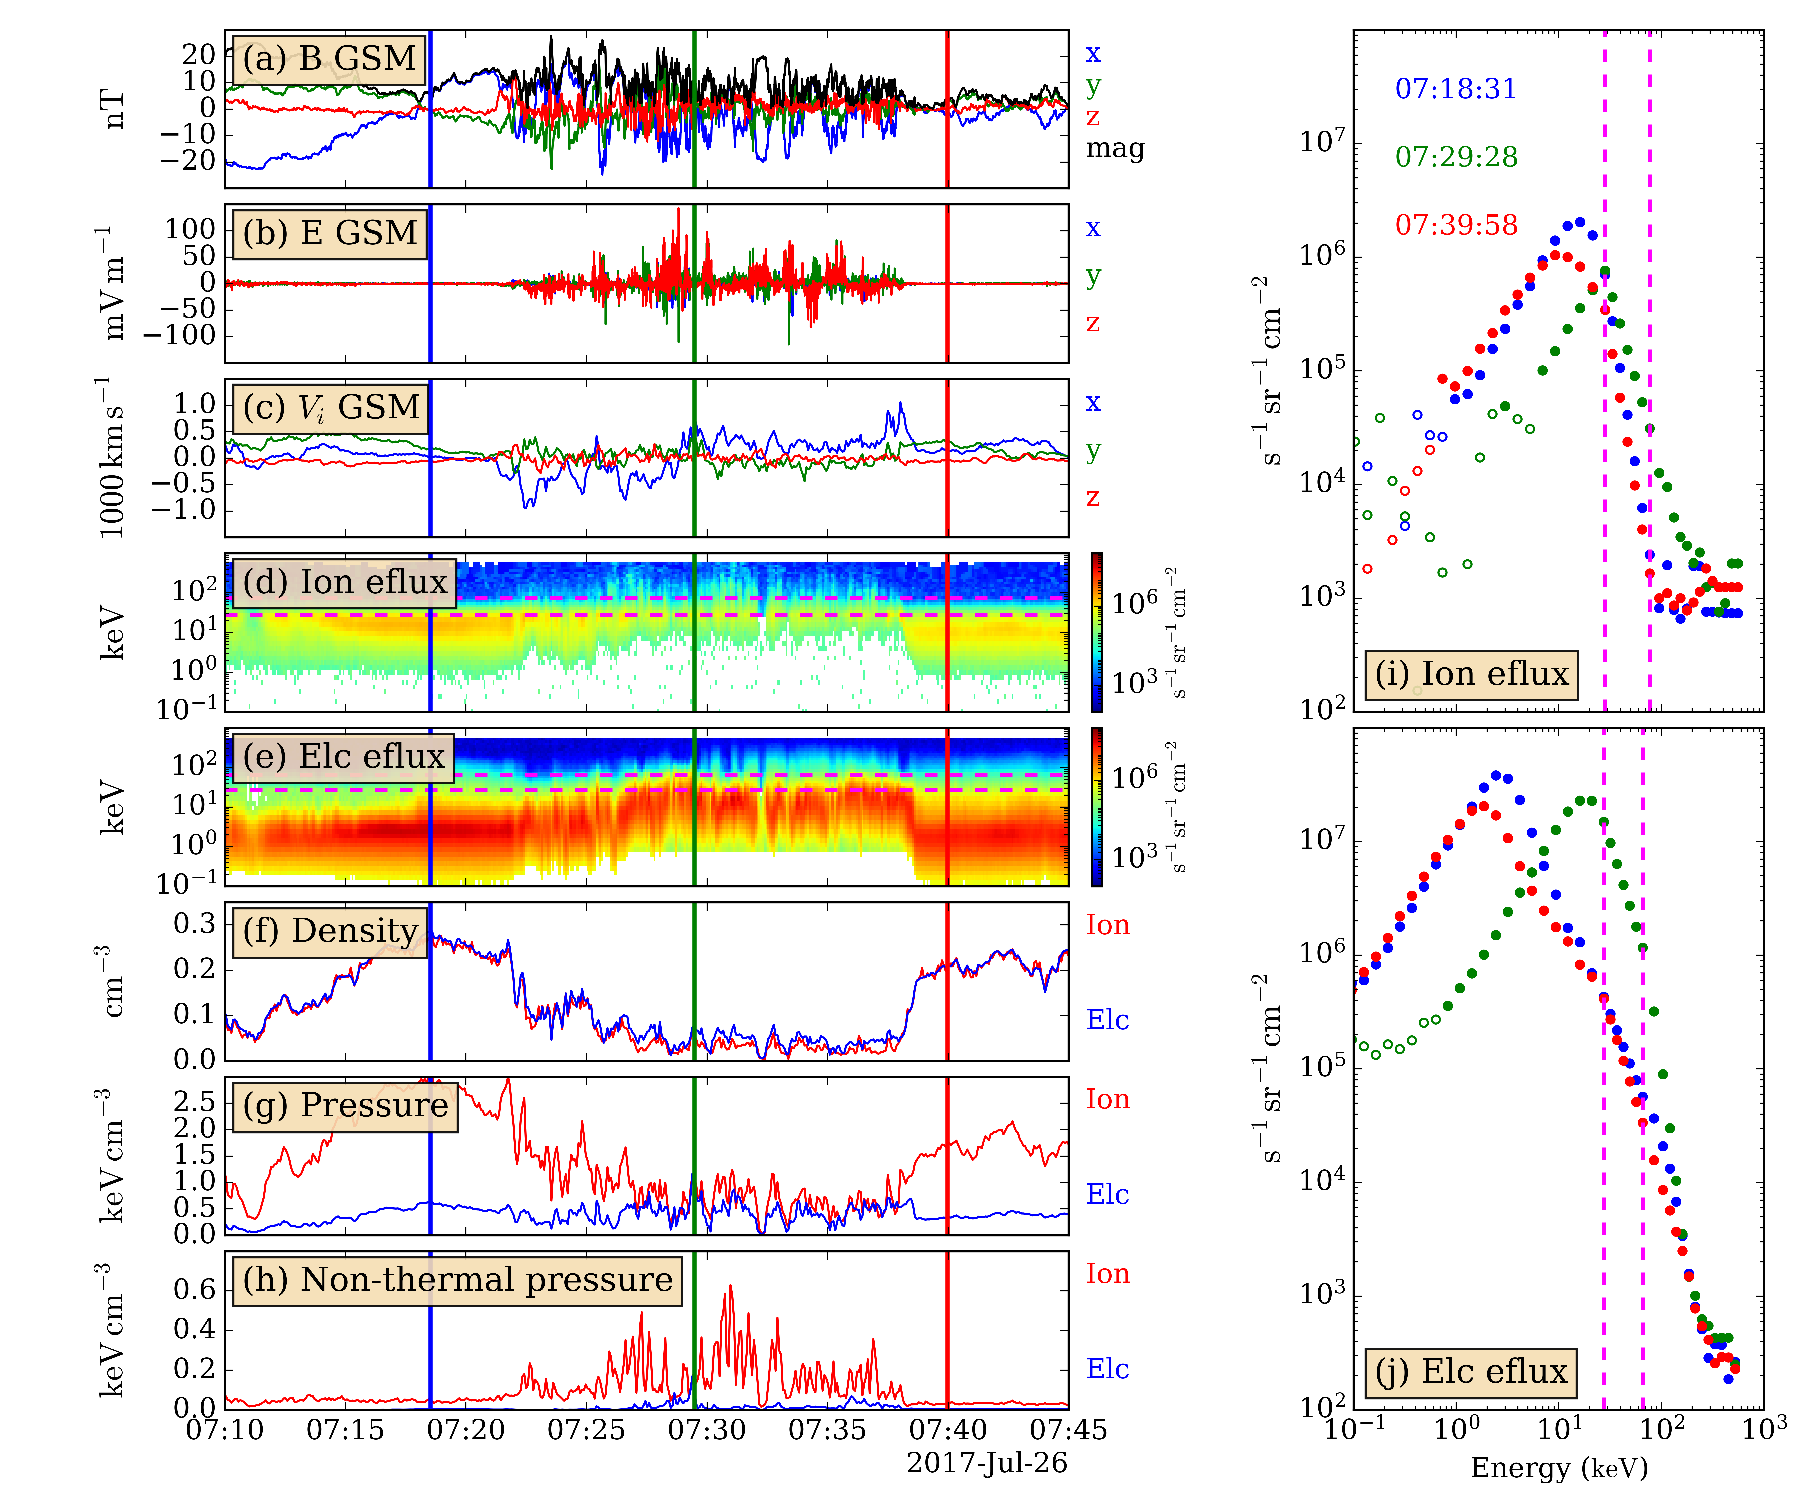
\includegraphics[width=\textwidth]{Fig1_fpi_feeps_combined_example.pdf}
\caption{
    Example of FPI-FEEPS combined moment calculations for a strong turbulent reconnection event in the magnetotail. (a) Barycentric magnetic field. (b) Barycentric electric field. The rest of the panels show data from MMS1. (c) Ion velocity. (d) Combined omni-directional ion \change{number}{energy} flux. (e) Combined omni-directional electron \change{number}{energy} flux. (f) Combined ion (red) and electron (blue) density. (g) Combined ion and electron total pressure. (h) Pressure contribution of non-thermal, energetic (larger than FPI energy threshold) particles. In (a-h), the blue, green, red vertical lines are times before, during, and after the turbulent event. (i) The ion \change{number}{energy} flux during vertical snapshots in (a-h). (j) Similarly, snapshots in electron \change{number}{energy} flux. \add{Hollow markers are noise-level or background measurements.} The dashed magenta lines [horizontal in (d) \& (e), vertical in (i) \& (j)] denote the extrapolated energy gap between FPI and FEEPS. There are 5 extrapolated points in that gap.
}
\label{fig:motivating_event}
\end{figure}

From past statistical studies \cite{Huang2020,Chong2022}, it is reasonable to assume that the plasma bulk flow rarely surpasses FPI capabilities (about 2,000\,\si{km/s} for ions and 100,000\,\si{km/s} for electrons). So the contribution from thermal (low-energy) particles to the plasma moments can be calculated from the FPI 3D distribution functions, correctly accounting for drifted particles. Subsequently, the non-thermal contribution may be considered isotropic and calculated from omni-directional distribution functions as detailed in \ref{appendix:combined_plasma_moments}. However, this calculation is limited to directionless quantities, such as the number density and scalar pressure. Most clearly seen in (i--j), the energy-coverage gap (between the dashed lines) may contain a significant contribution to the plasma moments. Thus, we extrapolate the distribution function in this gap from FPI and FEEPS measurements and include its contribution in the non-thermal moment calculations (see \ref{appendix:combined_plasma_moments}). In (f--h), we show the total (thermal + non-thermal) number density, total pressure, and non-thermal pressure.

In this event, one significant feature emphasized by the Ergun et al studies is that the reconnection inflow does not resupply particles from the lobe as fast as plasma sheet particles are depleted by the outflow, which results in a density drop in the turbulent region in (f) and the depletion of low-energy particles in (i--j). What we emphasize here is that because of this depletion of low-energy particles, when comparing (g) and (h), the contribution of non-thermal and/or energetic ions to the total pressure (characteristic energy density ${P_s=nk_BT_s}$ of species $s$) is on the order of 10\,\% and can be as high as 50\,\%. While most electrons are within the thermal (FPI) energy range, there can also be a significant fraction of non-thermal electrons ($\sim$ 10--20\,\% of total electron pressure) in this type of events. Since the frequency of events similar to the one shown in \cref{fig:motivating_event} is not yet established, pressure and temperature calculations solely based on the FPI instrument in the magnetotail may be underestimated for these occurrences. Therefore, it may be crucial for statistical studies of particle energization in the magnetotail to consider plasma moments combined from both FPI and FEEPS.

The calculation of combined plasma moments above requires that there is simultaneous availability from both particle instruments. We also require that electromagnetic field observations (from FGM and EDP) are available to enable future statistical studies of the correlation between field and particle observations. Such a study will be able to establish the statistical occurrence between turbulence, reconnection, and particle energization events such as the example in \cref{fig:motivating_event}.

For this study, we have compiled continuous intervals (no significant time gap; duration from minutes to hours) of good availability from the magnetic field, electric field, low-energy plasma, and energetic particle instruments during MMS magnetotail seasons from 2017 to 2020. Additionally, 1-minute averaged solar wind conditions are obtained from the OMNI dataset \cite{King2005}, which is used to correlate the magnetotail dynamics with solar wind conditions. In total, there are 437,728,300 field (FGM resolution) and 6,078,827 particle (FPI resolution) data points, amounting to about 316 continuous days of observation. Details of compilation of these intervals are highly technical and are laid out in the Supporting Information (SI). The principal conditions are listed below.
\begin{enumerate}
    \item ${X<0}$
    \item ${R\geq 12R_E}$
    \item ${Q\geq0.75}$
    \item No periods of thruster firing, EDP probe saturation, shadow spikes, or bad bias settings.
    \item FGM, EDP available from MMS(1--4).
    \item FPI, FEEPS available from MMS1.
    \item Interval at least 1-minute long.
\end{enumerate}
Above, ${\vb{R}=(X,Y,Z)}$ is the spacecraft position in GSM. While most global models of the neutral sheet, one of which is later on analyzed and compared, are fitted in aberrated GSM (AGSM), we have found little difference between GSM and AGSM in our results. Thus, we retain the usage of GSM for all coordinates in subsequent sections. Conditions (3) and (5) ensures that the barycentric electromagnetic fields and the curlometer current density may be accurately estimated. (4) ensures intervals of adequate EDP data for analysis. (6) ensures the partial plasma moments can always be combined. (7) enforces that the intervals are adequately long for spectral analysis.

\section{Properties of the magnetotail background plasma conditions}\label{sec:background_parameters}

In this section, we first distinguish the inner magnetotail from the solar wind and flank-side boundary layers, the properties of which are outside the scope of the present paper. Then, we present the statistical properties of the inner-magnetotail plasma conditions and compare our results with those in \citeA{Boakes2014}, hereby referred to as B14. Also, as done in B14, threshold conditions for the PS, PSBL, and lobe are derived based on the statistical properties of the plasma.

\subsection{Exclusion of solar wind and flank-side boundary layers}\label{sec:define_roi}

\begin{figure}
\centering
\noindent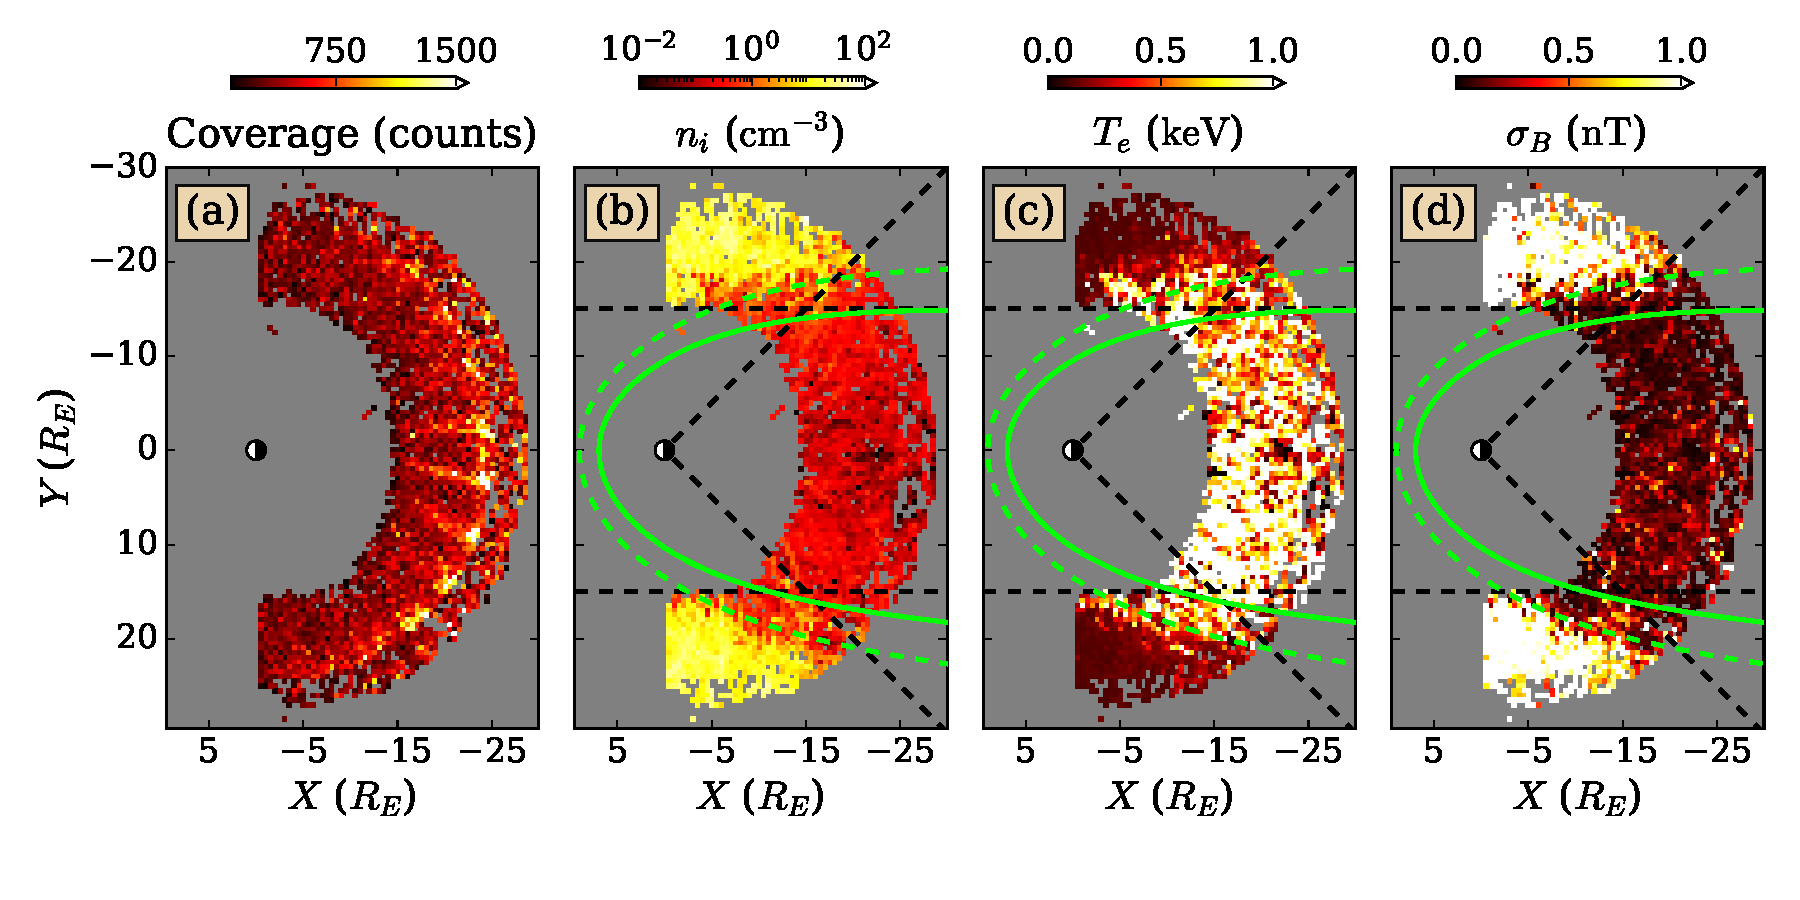
\includegraphics[width=\textwidth]{Fig2_inner_tail.pdf}
\caption{
Spatial distribution in the $X$--$Y$ plane of (a) MMS coverage during tail seasons in 2017--2020, (b) the ion density $n_i$, (c) the electron temperature $T_e$, and (d) standard deviation of the magnetic field $\sigma_B$. The lime curves are a $5^\circ$ (clockwise) tilted magnetopause model \cite{Lin2010} constructed with zero IMF $B_z$ and total solar wind pressure of 5\,\si{nPa} (dashed) and 20\,\si{nPa} (solid). Dashed black lines denote ${\abs{Y}\leq 15\,\si{R_E}}$ and ${\abs{Y}\leq\abs{X}}$. The color scales are chosen to saturate solar wind values to also reveal typical plasma values in the tail.
}
\label{fig:tail_roi}
\end{figure}

\cref{fig:tail_roi} shows the $X$--$Y$ distribution of (a) the coverage of MMS trajectory, (b) the ion density $n_i$, (c) the electron temperature $T_e$, and (d) the standard deviation of the magnetic field $\sigma_B$ (over a 5-s moving window). In the magnetotail, the electron density ($n_e$) measurement is more accurate than $n_i$. However, the reverse is true in the solar wind. Here, we use $n_i$ to reveal the differences between the solar wind and the magnetotail. Later, we use $n_e$ when characterizing the magnetotail. 3D histograms are calculated with ${0.5\,\si{R_E}\times0.5\,\si{R_E}\times0.5\,\si{R_E}}$ cubic bins then averaged over the $Z$ direction, except for (a), which is summed instead. Hereafter, all data (e.g. the magnetic field, electric field, and current density) are averaged over a 5-s moving window and subsequently down-sampled to FPI resolution (4.5\,\si{s}) so that particle and field measurements can be compared. Thus, in (a), each count represents a 5-s observation and the total count in each bin represents the dwell time of MMS spacecrafts. 3D bins that have lower than 100 counts are excluded as they may not be statistically representative.

In (a), the dwell time is not uniform. The highly-eccentric orbit has MMS spend more time near the apogee to maximize the chance of observing the diffusion region at reconnection sites \cite{Fuselier2016}. However, bins that have statistically significant counts are distributed over a large and uniform enough area so that the spatial distribution of plasma parameters can be studied. Most notably in (b--d), the solar wind is observed (as saturated colors) at ${\abs{Y}\gtrsim15\,\si{R_E}}$, where averaged values are ${n_i\sim}$ 10--100\,\si{cm\tothe{-3}}, ${\sigma_B\sim}$ 1--5\,\si{nT}, and ${T_e\sim}$ 0.01--0.1\,\si{keV}. In contrast, plasma parameters in the inner magnetotail are generally 1--2 orders of magnitude smaller, where ${n_i\sim}$ 0.1--1\,\si{cm\tothe{-3}}, ${\sigma_B\sim}$ 0.1--0.5\,\si{nT}, and ${T_e\sim}$ 1\,\si{keV}. \change{This figure}{\mbox{\cref{fig:tail_roi}}} shows that in general, background plasma parameters such as the density, temperature, and magnetic field fluctuations are distinctive between the inner and outer magnetotail. Thus, we can use these differences to statistically exclude regions more likely associated with the solar wind or flank-side boundary layers.

OMNI solar wind observations during MMS magnetotail seasons indicate average IMF ${B_z\sim0}$ and total pressure ${P_\text{sw}\sim}$ 1--5\,\si{nPa}. We use these parameters to construct an asymmetric magnetopause model \cite{Lin2010}, plotted as dashed (${P_\text{sw}=5\,\si{nPa}}$) and solid (${P_\text{sw}=20\,\si{nPa}}$) lime curves in (b--d). Details about the average OMNI observations and the Lin10 model are provided in \ref{appendix:omni}. The dashed curve agrees well with the change in plasma parameters. Thus, to be conservative when eliminating boundary layers, we define the inner magnetotail as the region bounded by the solid lime curve. In subsequent sections, all statistical results are obtained with data located strictly within this region.

For comparison, previous statistical studies have typically constrained the inner magnetotail region either with (i) ${\abs{Y}\leq\abs{X}}$ \cite{Ergun2015} or (ii) with a threshold ${\abs{Y}\leq Y_0}$ \cite{Boakes2014,Chong2022}. These two constraints are plotted as dashed black lines in (b--d). On a closer look, they are all somewhat equivalent conditions. (i) tends to work for smaller radial distances ${R\leq12\,\si{R_E}}$, and (ii) is good for small enough threshold $Y_0$, although the popular choice ${Y_0=15\,\si{R_E}}$ may include some mixed plasma data. 

\subsection{Identification of inner tail plasma
environments}\label{sec:tail_environments}

\begin{figure}
\centering
\noindent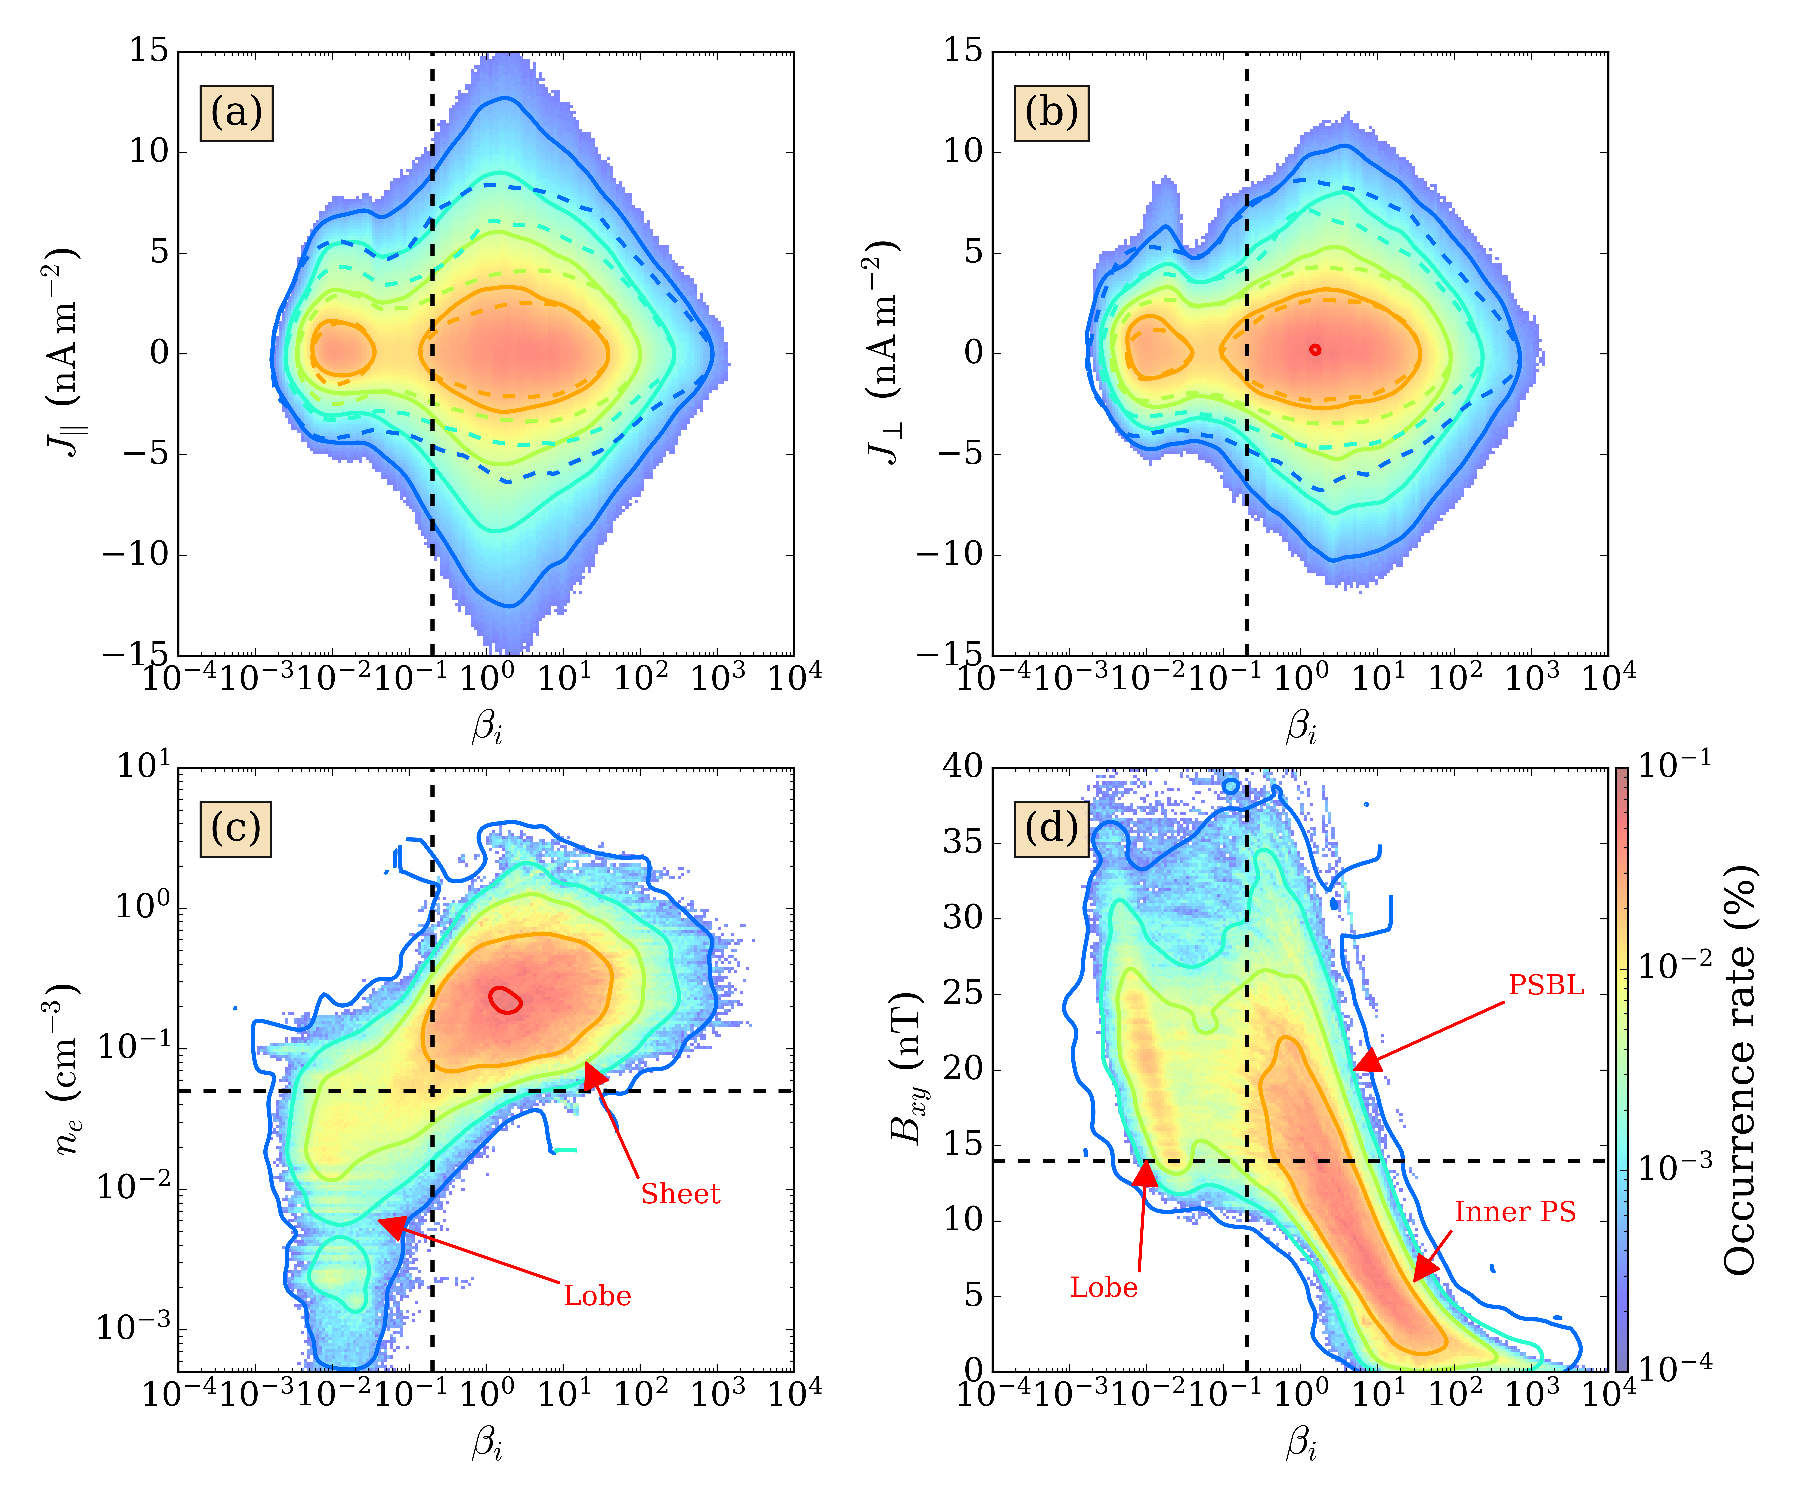
\includegraphics[width=\textwidth]{Fig3_compare_B14.pdf}
\caption{
    \change{Statistical distribution}{Occurrence rates} of (a) the parallel current density $J_\|$, (b) the perpendicular current density $J_\perp$\add{ (in the cross-tail direction, ${\hat{\vb{z}}\cross\vb{B}}$)}, (c) the electron density $n_e$, and (d) the equatorial magnetic field $B_{xy}$ in terms of the ion plasma beta $\beta_i$. \add{Solid lines are contours of the colored distributions. In (a) and (b), the overplotted colored dashed lines are contours of the noise estimation of the curlometer current, ${\div{\vb{B}}/\mu_0}$.} In all panels, the vertical dashed line denotes ${\beta_i=0.2}$. In (c), the horizontal dashed line is the FPI 1-count level ${n_e=0.05\,\si{cm\tothe{-3}}}$. In (d), the horizontal dashed line denotes ${B_{xy}=14\,\si{nT}}$. \remove{The current and magnetic field measurements are down-sampled to FPI resolution in this figure.}
}
\label{fig:compare_B14}
\end{figure}

\cref{fig:compare_B14} shows the statistical profile of background plasma parameters in terms of the ion beta ${\beta_i=P_i/(B^2/2\mu_0)}$, where $P_i$ is the ion pressure. For comparison, it is plotted in the same format as Figure 1 in B14. (a) and (b) show the current density components parallel ($J_\|$) and perpendicular ($J_\perp$) to the background magnetic field. (c) shows the electron density $n_e$, and (d) shows the equatorial magnetic field $B_{xy}$. \remove{Similar to \mbox{\cref{fig:tail_roi}(a)}, each count represents a 5-s observation.} \add{Due to the solenoidal condition (\mbox{${\div{\vb{B}}=0}$}), the noise level of the curlometer currents in (a--b) can be estimated as \mbox{${J_\text{noise}=\div{\vb{B}}/\mu_0}$}. In these panels, we have overplotted the contours of \mbox{$J_\text{noise}$} for comparison with the current amplitude. At a given color, currents larger than noise are measured if the solid line is wider than the dashed line.}

In general, the features in this plot are consistent with the Cluster study. Most clearly in all panels, there are two distinct populations separated by $\beta_i$. The lobe-like population has low density (${n_e\sim0.01\,\si{cm\tothe{-3}}}$), low beta (${\beta_i\sim0.01}$), and high equatorial magnetic field (${B_{xy}\sim20\,\si{nT}}$). In contrast, the plasma sheet-like population has high density (${n_e\sim0.1\,\si{cm\tothe{-3}}}$), high beta (${\beta_i\sim1}$), and low field (${B_{xy}\sim5\,\si{nT}}$). One note of caution is the region of low electron density. The FPI instrument has a large uncertainty if the electron density is below \mbox{0.05\,\si{cm\tothe{-3}}} [horizontal dashed line in (c)]. \add{However, noise and background in the combined FPI-FEEPS distribution function has been treated carefully in the low-density region such that the accuracy is improved (see \mbox{\ref{appendix:combined_plasma_moments}} for details).} In subsequent sections, the threshold conditions for the plasma sheet are the main subject of study, where the density is typically higher than \change{this}{the FPI} threshold. \remove{While it is possible that there are unusually low-density plasma in the PS, such as a few data points during the turbulent event in \mbox{\cref{fig:motivating_event}}, the occurrence is brief and does not significantly alter the results of a large statistical study.}

\begin{table}
\caption{Threshold conditions distinguishing tail plasma environments derived from \cref{fig:compare_B14}.}
\label{tab:threshold_conditions}
\centering
\begin{tabular}{l c}
\hline
 Plasma environment             & Condition  \\
\hline
  Lobe                          & ${\beta_i<0.2}$  \\
  Plasma sheet                  & ${\beta_i\geq0.2}$ \& ${B_{xy}\leq14\,\si{nT}}$  \\
  Plasma sheet boundary layer   & ${\beta_i\geq0.2}$ \& ${B_{xy}>14\,\si{nT}}$  \\
\hline
\end{tabular}
\end{table}

To systematically determine the thresholds, B14 used changes in the current and electron densities with respect to $\beta_i$ to define the PS/lobe separation and similarly, the statistical spread in $B_{xy}$ to distinguish between the PSBL and the outer/inner regions of the plasma sheet. The threshold conditions were then reported annually. However, we deem it unnecessary for that level of detail in this study. It suffices to define by visual inspection the threshold conditions as tabulated in \cref{tab:threshold_conditions} and annotated in \cref{fig:compare_B14}. We also make no attempt to distinguish the inner PS from the outer PS as done in B14. In general, our thresholds are all consistent with averages from the yearly results in B14. The beta threshold is slightly higher (by a factor of 2), most probably due to the usage of combined plasma moments (only partial moments with energies $\lesssim$ 40\,\si{keV} were used in the B14 study).

\begin{figure}
\centering
\noindent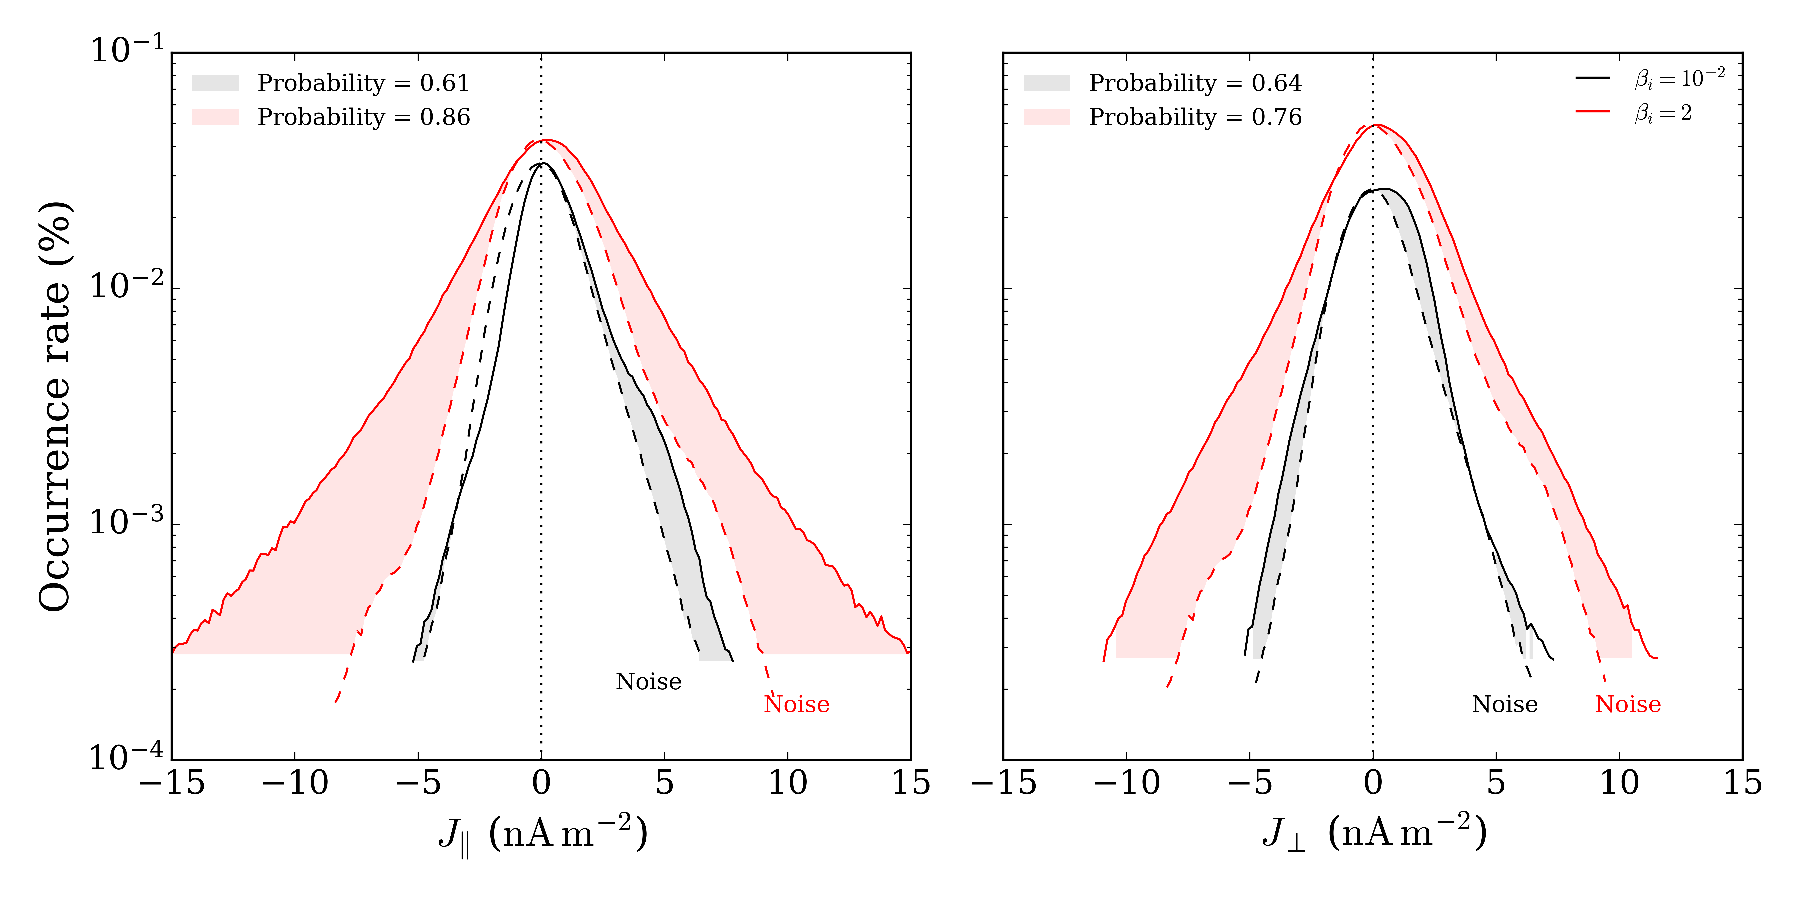
\includegraphics[width=\textwidth]{Fig4_J_slices.pdf}
\caption{
    Vertical cuts of the statistical distribution of the currents in \cref{fig:compare_B14}(a--b) at ${\beta_i=10^{-2}}$ (in black) and ${\beta_i=2}$ (in red). The corresponding dashed lines with the same colors are the noise estimation $J_\text{noise}$. The shaded areas are those where more occurrence is observed at a given amplitude than the noise estimation. The probability of these observations based on the shown conditional distribution functions (on $\beta_i$) is provided in the legends (shaded area versus total area under the solid lines).
}
\label{fig:J_slices}
\end{figure}

\change{
    A significant difference between our results and the B14 results is the current density. In (a) and (b), stronger currents $\sim$ \mbox{1.5--5\,\si{nA/m\tothe{2}}} are observed, while the current amplitude in B14 is $\sim$ \mbox{0.5--2\,\si{nA/m\tothe{2}}}. While B14 only observed noise-level lobe currents $\sim$ \mbox{0.1\,\si{nA/m\tothe{2}}}, this study reveals significant lobe currents with amplitude comparable to those in the PS and PSBL. Additionally, the parallel component in (a) averages to zero, indicating that the current frequently propagates obliquely with respect to the background magnetic field in both the lobe and PS. This also shows that the plasma is often frozen into the magnetic field.
}{
    In (a) and (b), the average current amplitude in the PS is consistent with results in B14 (\mbox{0.5--2\,\si{nA/m\tothe{2}}}). However, a difference among our results is in the lobe (low-beta region). B14 only observed noise in this region (\mbox{$J\sim0.5\,\si{nA/m\tothe{2}}$}). But the wider (green/blue) contours than \mbox{${J_\text{noise}}$} show that there are detections of statistically significant lobe currents above the noise level. To better visualize this difference, \mbox{\cref{fig:J_slices}} shows vertical cuts of these panels at \mbox{$\beta_i=10^{-2}$} (black) and \mbox{$\beta_i=2$} (red). The occurrence rate of high-beta currents is higher than those with low \mbox{$\beta_i$}. The shaded regions indicate that there are ``wings'' in the probability distribution functions (PDFs) that is more significant than the statistics of noise (dashed lines). At any occurrence rate below \mbox{$2\times10^{-3}\,\%$} for low $\beta_i$, the detected current amplitudes are higher than the estimated noise, which means wider contours in \mbox{\cref{fig:compare_B14}}. Finally, to show the partition between noise-level currents (in the ``core'' of the PDFs) and non-noise currents (in the wings), we calculate the probability of the latter (see the figure legends) and discover that at least half of the observations are not noise. That said, the low overall occurrence rate indicates that their detection is not common.
}

\remove{An explanation for the discrepancy in current amplitude lies in the average spacecraft separation. }In the magnetotail, the typical Cluster spacecraft separation is 1000s of \si{km} \cite{Escoubet2001}, which is comparable to the average ion inertial length. About ${\sqrt{m_i/m_e}\sim40}$ times smaller, the typical electron inertial length is ${\sim20\,\si{km}}$. Since the target of MMS is electron physics, 97\,\% of the dataset has spacecraft separation ${\leq70\,\si{km}}$ (not shown). As a result, intense electron-scale currents are resolved in MMS data, but may be underestimated in Cluster data due to the linear spatial interpolation in the curlometer technique \cite{Paschmann1998}. \remove{This can explain the higher average amplitude in MMS observations}. \add{Therefore, we hypothesize that the presence of significant lobe currents in our statistics is due to the smaller spacecraft separation. Future studies are necessary to reveal their origin and properties. }Overall, these results still provide strong support of Cluster observations from the MMS mission, with an improvement on current density measurements.

\section{Global structure of the magnetotail plasma sheet}
\label{sec:global_structure}

In this section, we investigate the three-dimensional global structure of the plasma sheet. As mentioned in \cref{sec:intro}, the magnetotail is influenced by processes such as flapping, twisting, and warping. Therefore, the plasma sheet may be highly deformed on mesoscales. In that case, it is interesting to study the spatial variations of the background plasma conditions, based on which the PS threshold condition is established in \cref{tab:threshold_conditions}. From solar wind observations in \ref{appendix:omni}, the average IMF $B_y$ is around 2\,\si{nT} with near-zero IMF $B_z$, suggesting that the twisting angle should not be significant for radial distances smaller than 30\,\si{R_E} \cite{Tsyganenko2004}, which leaves flapping and warping as the main deforming factors during MMS magnetotail seasons.

To investigate the warping of the magnetotail plasma sheet, we consider the Earth's dipole tilt angle $\Psi$ obtained from the MMS Magnetic Ephemerides Coordinates (MEC) dataset generated by \citeA{Henderson2018}. In GSM coordinates, $\Psi$, constrained in the $X$--$Z$ plane, is the angle between the Earth's dipole tilt axis and the $Z$ axis, which is positive when the Earth tilts toward the Sun and negative away from the Sun. Due to the daily Earth rotation, $\Psi$ varies almost sinusoidally with an amplitude of about ${10^\circ}$ and a period of about 1 day (not shown). \cref{fig:tilt_distribution} shows the distribution of $\Psi$ with respect to (a) the time of year and (b) the concurrent MMS spacecraft position in $Y$. 

\begin{figure}
\centering
\noindent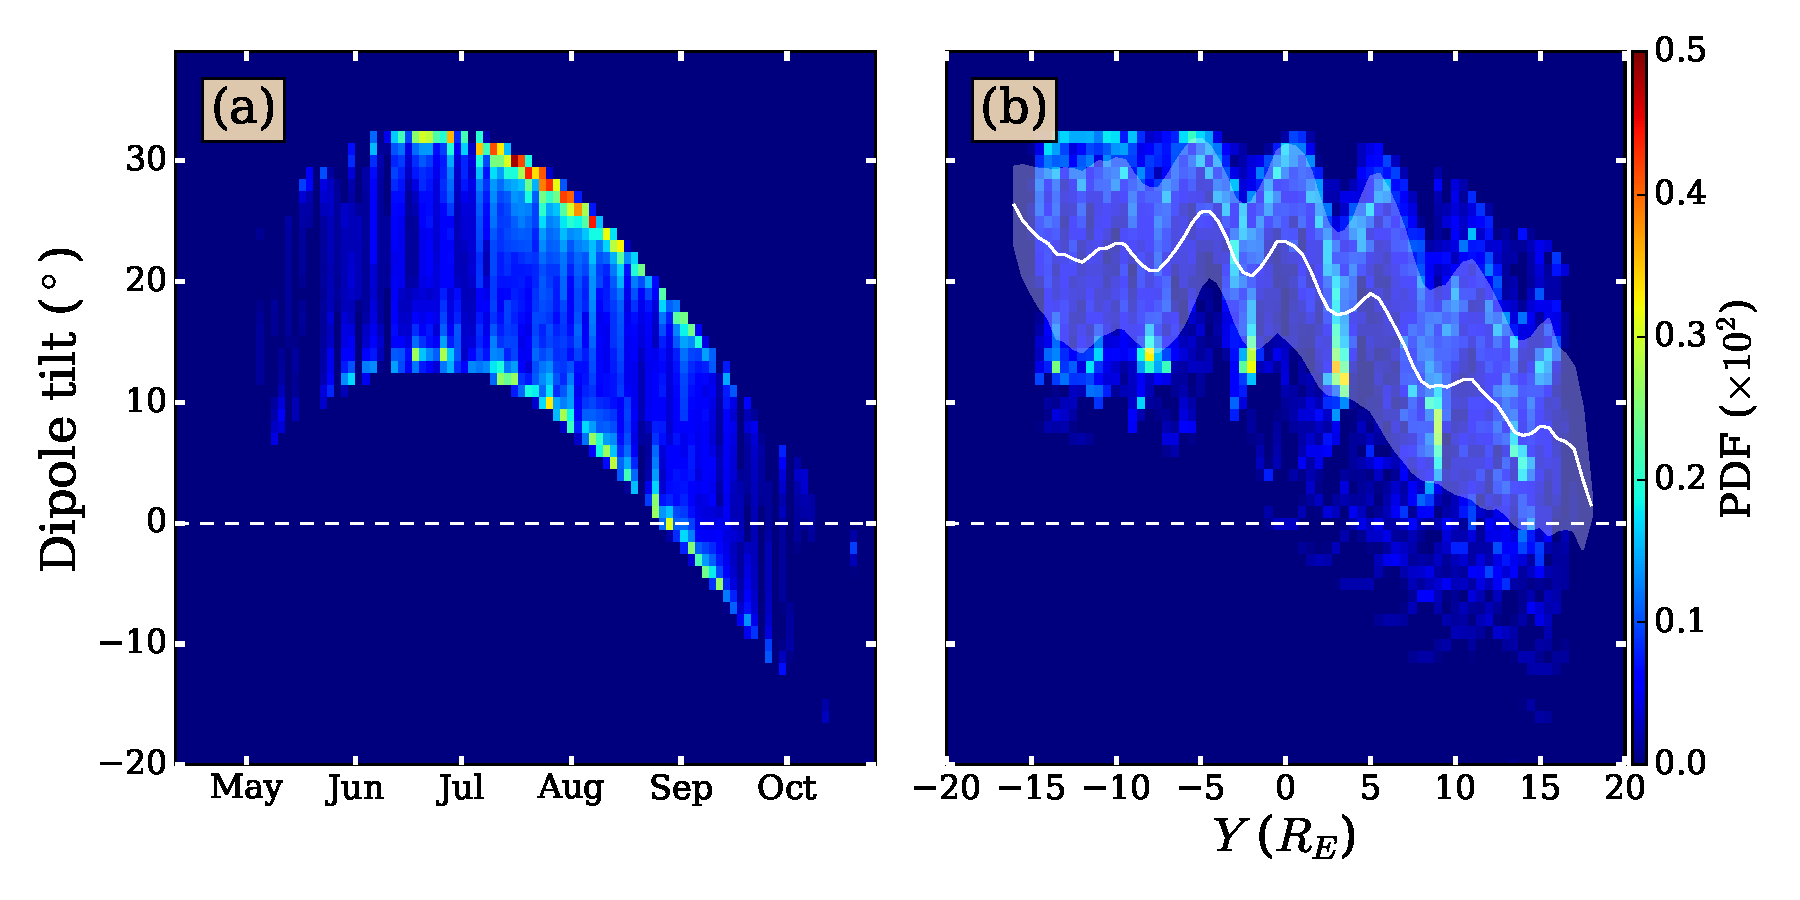
\includegraphics[width=\textwidth]{Fig5_dipole_tilt.pdf}
\caption{
Distribution of the dipole tilt angle $\Psi$ (a) in time and (b) in $Y$. The average $\Psi$ is plotted as the solid white line in (b).
}
\label{fig:tilt_distribution}
\end{figure}

In (a), there are two peaks separated by $\sim20^\circ$ due to the daily variation of $\Psi$ and the seasonal variation of the dipole tilt ($\Psi$ is lower in October). The daily variation is also seen in panel (b). However, (b) also shows that $\Psi$ is lower at higher $Y$. The correlation between $\Psi$ and $Y$ is due to low natural precession of the MMS orbit, which causes MMS to visit the magnetotail only in the summer months. In these seasons, MMS enters the magnetotail from the dawn-side flank (${Y\sim-15\,\si{R_E}}$) around May when $\Psi$ is high and exits to the dusk-side flank (${Y\sim15\,\si{R_E}}$) around October when $\Psi$ is low. The solid white line in (b) shows the average value of $\Psi$ in terms of $Y$, which is around $20^\circ$ in the dawn sector (${Y<0}$) and gradually decreases to zero in the dusk sector (${Y>0}$). The difference in average $\Psi$ between these two sectors can lead to significant variations as a function of $Y$ due to dipole tilt warping effects.

Using the same bin size as that in \cref{fig:tail_roi} (0.5\,\si{R_E}),
\change{\mbox{\cref{fig:XZ,fig:YZ}} show the spatial variations of several background parameters in both the $X$-$Z$ and $Y$-$Z$ plane (the third dimension is averaged in both cases), thereby providing a 3D picture of these quantities. In \mbox{\cref{fig:XZ}}, we show (a) the ion plasma beta $\beta_i$, (b) the equatorial magnetic field $B_{xy}$, and (c) the normal electric field $E_z$.}{\mbox{\cref{fig:XZ}} shows the ($Y$ averaged) spatial structure of (a) the ion plasma beta $\beta_i$, (b) the equatorial magnetic field $B_{xy}$, and (c) the normal electric field $E_z$. Similarly, \mbox{\cref{fig:YZ}} shows the ($X$ averaged) spatial structure of (a) $B_x$ and (b) $\Psi$. The structures of these parameters altogether provide a 3D picture of the plasma sheet, with the tilt angle $\Psi$ indicating the degree of warping.}

In \change{each panel}{\mbox{\cref{fig:XZ}}} from (a) to (c), the bins are marked with a dot if they satisfy the beta condition, the magnetic field condition, and both (the plasma sheet condition in \cref{tab:threshold_conditions}), respectively. The features in this figure correspond one-to-one with those discussed in \cref{tab:threshold_conditions}. First, in \cref{fig:XZ}(a), while constraining $\beta_i$ to high values mostly excludes environments consistent with the lobe, the PSBL and PS can extend widely in $Z$. So the beta condition does not reveal much about the spatial extent. In \cref{fig:XZ}(b), the magnetic field condition excludes the PSBL regions, leaving the remaining PS, which is more narrow along ${Z=0}$. In \cref{fig:XZ}(c), the normal electric field $E_z$ that supports the cross-tail drift current ${J_y\propto-E_zB_x}$ also roughly follows this spatial structure. This electric field always points towards the inner PS (negative/positive in the northern/southern lobe) and tends to zero at the NS. This plot shows that the PS threshold condition agrees with the spatial structure of the PS, as drawn out by the normal electric field ($E_z$) and equatorial magnetic field ($B_{xy}$).

\begin{figure}
\centering
\noindent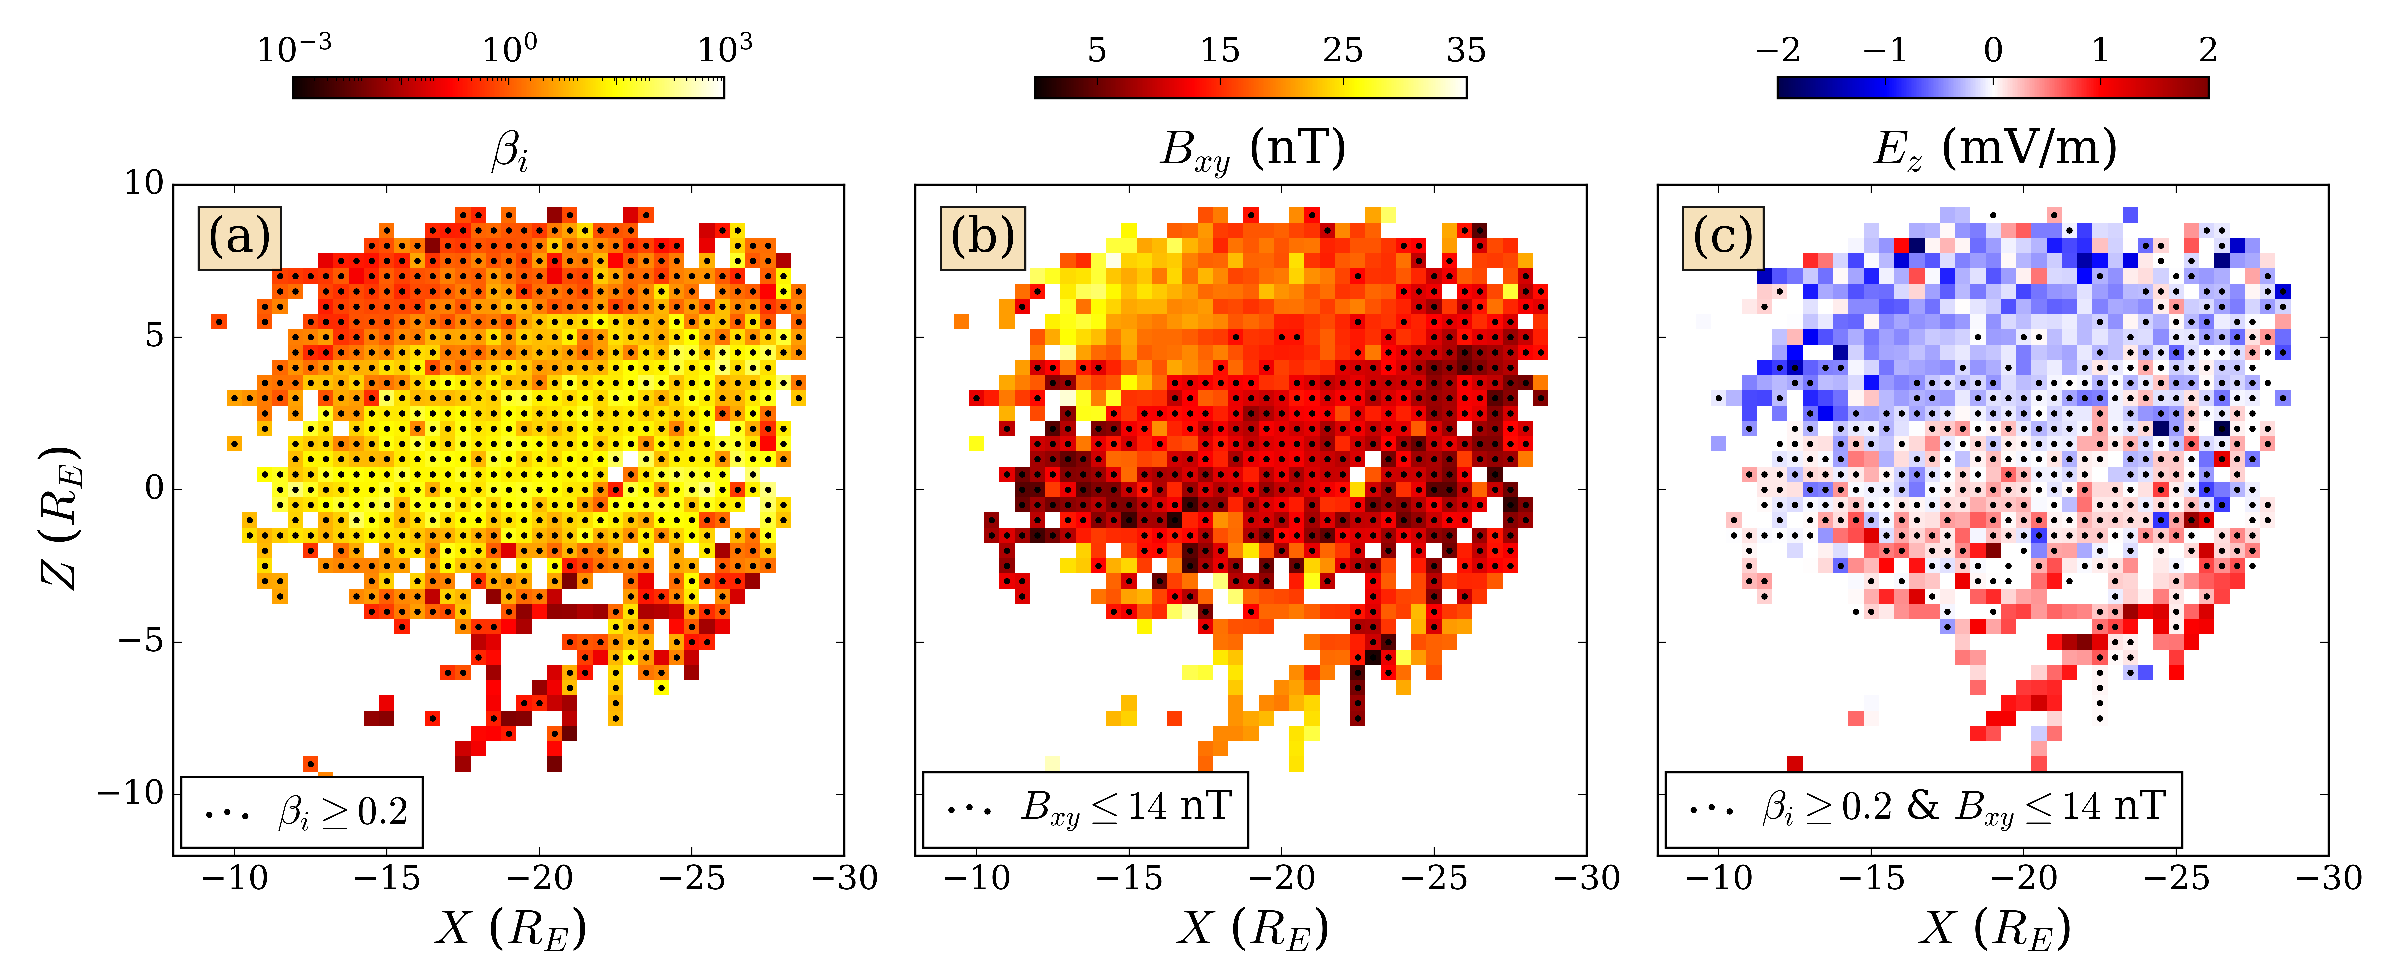
\includegraphics[width=\textwidth]{Fig6_XZ_distribution.pdf}
\caption{
Spatial distribution in the $X$--$Z$ plane of (a) $\beta_i$, (b) $B_{xy}$, and (c) $E_z$. In (a), marked bins (those with a circle marker at the center) satisfy the PS beta condition ${\beta_i\geq0.2}$ in \cref{tab:threshold_conditions}. Similarly, the marked bins satisfy the PS field condition ${B_{xy}\leq 14\,\si{nT}}$ in (b). Those in (c) satisfy both, the full PS condition.
}
\label{fig:XZ}
\end{figure}

The spatial extent of $E_z$ in the $Z$ direction seemingly flares up to $\sim$ 8--10\,\si{R_E} beyond ${\abs{X}\gtrsim20\,\si{R_E}}$, \change{but}{while} at closer distances, its structure is mainly located within 5\,\si{R_E} of the equator. This flaring in the $Z$ direction of the plasma sheet can be explained with variations in the $Y$ direction caused by the dipole tilt. \change{\mbox{\cref{fig:YZ}} shows (a) the magnetospheric $B_x$ component and (b) the dipole tilt angle $\Psi$ in the $Y$-$Z$ plane. The two lobes are clearly distinguishable in (a)}{In \mbox{\cref{fig:YZ}(a)}, the two lobes are clearly distinguishable}, with ${B_x>0}$ indicating the northern hemisphere and ${B_x<0}$ indicating the southern hemisphere. The null point ${B_x\sim0}$ is the location of the neutral sheet. In (b), the distribution of $\Psi$ also reflects the aforementioned dawn-dusk asymmetry in \mbox{\cref{fig:tilt_distribution}}, where $\Psi$ varies between 10$^\circ$ and 30$^\circ$ in the dawn sector ($Y<0$) and between -10$^\circ$ and 10$^\circ$ in the dusk sector ($Y>0$).

\begin{figure}
\centering
\noindent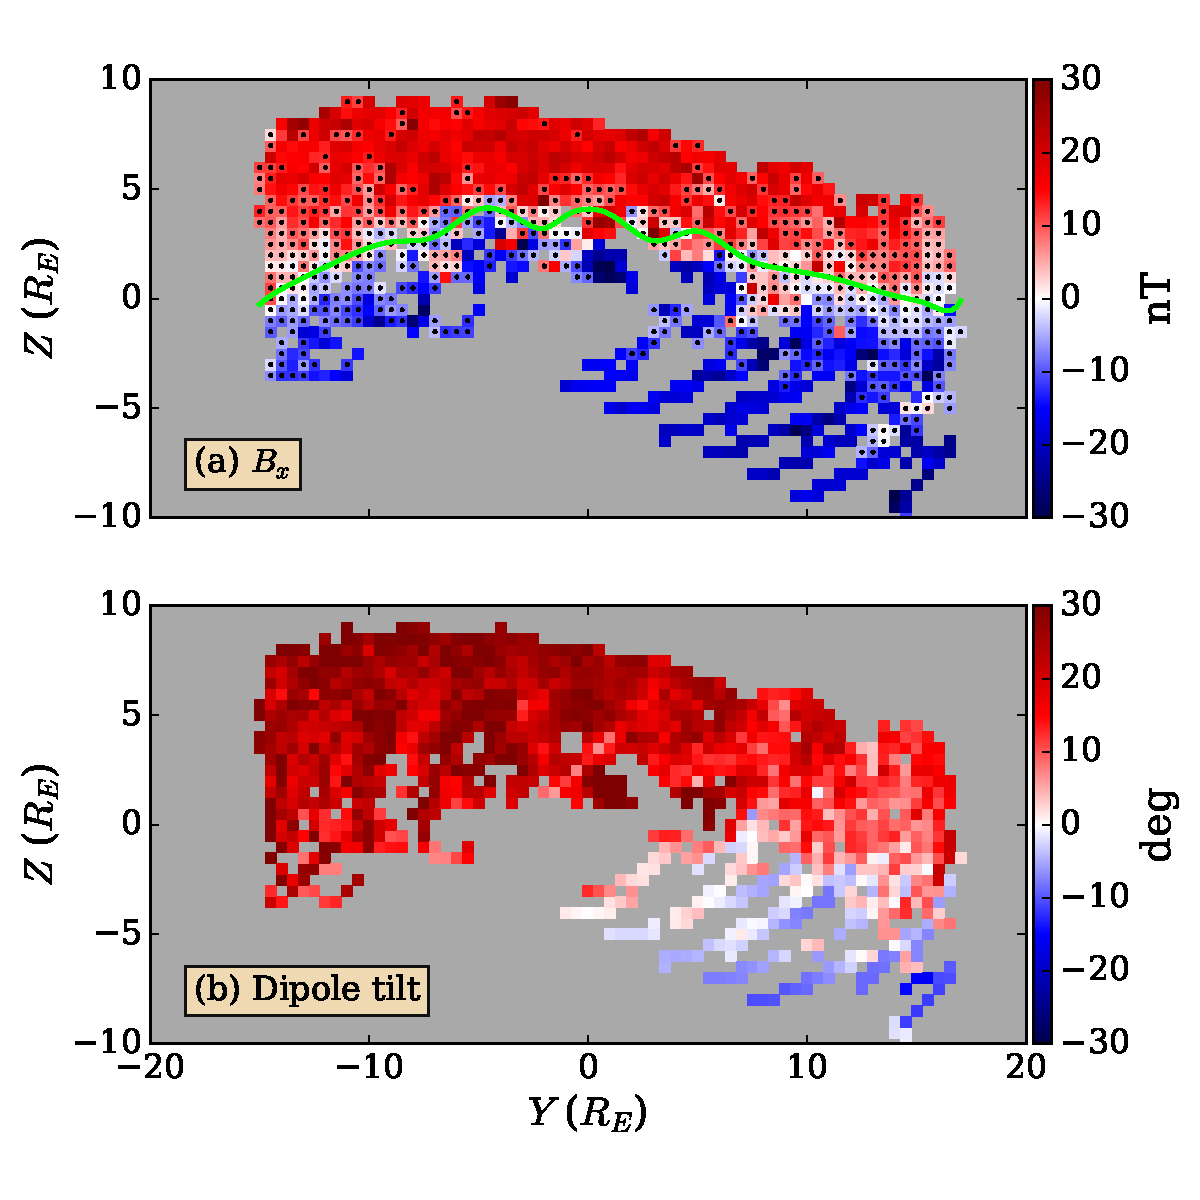
\includegraphics[width=\textwidth]{Fig7_YZ_distribution.pdf}
\caption{
Spatial distribution in the $Y$--$Z$ plane of (a) $B_x$ and (b) the dipole tilt angle $\Psi$. The solid lime line in (a) is a global tail neutral sheet model \cite{Xiao2016} dependent on $\Psi$ and the average solar wind pressure $P_\text{sw}=2\,\si{nPa}$. Similar to \cref{fig:XZ}(c), the marked bins satisfy the plasma sheet condition  (plotted in the same format).
}
\label{fig:YZ}
\end{figure}

%\remove{In the same format as \mbox{\cref{fig:XZ}}, }\change{b}{B}ins marked with a dot in \cref{fig:YZ}(a) indicate the \change{plasma sheet region}{region satisfying the PS condition in \mbox{\cref{tab:threshold_conditions}}}. The reversal of $B_x$ shows that the neutral sheet is located within the marked plasma sheet. The lime curve is a global NS model from \citeA{Xiao2016}, dependent on the dipole tilt angle and the solar wind pressure (see \ref{appendix:omni}). We use the average value of $\Psi$ obtained from \cref{fig:tilt_distribution}(b) (solid white line) for the former, and average OMNI observations ${P_\text{sw}=2\,\si{nPa}}$ for the latter. The small variations in this model are highly dependent on those in $\Psi$, which in turn is affected by the spacecraft apogee. However, its average shows a remarkable agreement with the $B_x$ reversal. 
%
%In \cref{fig:YZ}(b), the high values of $\Psi$ in the dawn sector causes the magnetotail to be warped to $\sim$ 2--4\,\si{R_E} in $Z$, while in the dusk sector, there is little warping. The combination of warping in the dusk sector with no warping in the dawn sector contributes to the apparent flaring in $X$--$Z$ seen in \cref{fig:XZ}, as the $Y$ direction is averaged in that figure. The plasma sheet extent around the neutral sheet in \cref{fig:YZ}(a) seems to increase towards the flanks ($\sim$ 2--3\,\si{R_E}). This increase may be explained by kink-like flapping waves that are commonly observed in these regions \cite{Gao2018}. As the magnetic field condition is more strictly constrained to lower threshold, the outer PS is excluded and will result in a spatial distribution that follow the NS more closely.
%
%\section{Discussions and Conclusions}\label{sec:conclude}
%
%In summary, using a large volume of MMS data with combined plasma moments from the low-energy plasma and energetic particle instruments, we have investigated the background plasma conditions and the 3D spatial structure of the magnetotail plasma sheet using the threshold, imaging, and modeling approaches. Consequently, we have statistically distinguished inner-magnetotail environments corresponding to the plasma sheet, plasma sheet boundary layers, and lobes. We find that these methods are in good agreements, showing that the neutral sheet is embedded within a thick region of the plasma sheet, and they are both highly warped in the dawn sector and less deformed in the dusk sector.
%
%This asymmetry is attributed to changes in the dipole tilt angle as the Earth orbits the Sun (see \cref{fig:tilt_distribution,fig:YZ}). But this observation is, in part, also specific to MMS, since the mission always visits the magnetotail in the summer months due to its orbital design. \cref{fig:sketch} provides a schematic of the Earth's magnetospheric configurations during these periods. As MMS enters the magnetotail from the dawn-side flank around June solstice, the Earth's dipole on average tilts around $20^\circ$ towards the Sun, resulting in a highly warped neutral sheet at $Z\sim$ 2--4\,\si{R_E} [see \cref{fig:YZ}(a)]. But when it exits the magnetotail from the dusk-side flank around September equinox, the average tilt angle is zero, leading to a less deformed and displaced neutral sheet. 
%
%\begin{figure}
%\centering
%%\noindent\includegraphics[width=\textwidth]{resources/figures/schematic-v7.pdf}
%%\caption{
%%    Schematic of Earth's magnetospheric configurations during an MMS magnetotail season. \change{Around June solstice, MMS (green dots) enters from the dawn side when the magnetotail is highly warped in the positive $Z$ direction. Also around this time, the Earth's dipole tilt (solid blue arrow) angle fluctuates between $10^\circ$ and $30^\circ$ on a daily basis, averaging at $20^\circ$ towards the Sun. Around September equinox, MMS exits from the dusk side when the magnetotail is less displaced from the equator. Here the average dipole tilt angle is zero.}{The Earth's rotational axis ($\Omega$, dashed yellow) is constant. The magnetic dipole moment (solid blue arrow) rotates around this axis once a day, warping the magnetotail up and down in $Z$ GSM. Around June solstice, MMS (green dots) enters the magnetotail from the dawn side. During this period, GSM (red) coincides with GSE (white) coordinates whenever the moment lies in the XZ plane. The tilt angle is large, resulting in a highly warped magnetotail in the positive $Z$ direction. Towards September equinox, MMS exits the magnetotail from the dusk side. During this period, whenever the moment lies in the YZ plane, the Z axis of GSM coordinate is parallel with the dipole moment. The small tilt angle results in a relaxed magnetotail.}
%%}
%\label{fig:sketch}
%\end{figure}
%
%While we have demonstrated that the deformation of the magnetotail mainly comes from warping, there remains flaring effects due to kink-like flapping waves or IMF twisting near the flanks that are not discussed in details in this paper. Future studies may need to consider smaller-scale evolution and utilize timing analysis to investigate properties of the flapping in further details. However, the insights about the plasma sheet spatial variations reported in this paper will be useful for future MMS magnetotail studies when considering its configuration and the state of the plasma sheet.
%
%The threshold conditions in \cref{fig:compare_B14} and \cref{tab:threshold_conditions} are also in good agreement with a previous Cluster study \cite{Boakes2014}. \change{However, a few improvements are made. First, the current density estimation using the curlometer technique \mbox{\cite{Paschmann1998,Dunlop2021}} is inherently improved, due to the MMS mission design with smaller average spacecraft separation in the magnetotail. Higher-amplitude currents in the PS and significant currents in the lobes are frequently observed because thin electron-scale currents are resolved [\mbox{\cref{fig:compare_B14}(a--b)}]. Second,}{The average current amplitude in the PS agrees with Cluster observations. However, lobe currents with amplitude comparable to those in the PS are also detected, albeit their occurrence rate is lower [\mbox{\cref{fig:compare_B14}(a--b)}, \mbox{\cref{fig:J_slices}}]. One interpretation of their presence is that thin electron-scale currents are resolved in the curlometer calculation due to MMS mission design with smaller average spacecraft separation in the magnetotail \mbox{\cite{Paschmann1998,Dunlop2021}}. While small-scale current systems have been observed with Cluster via the particle distribution function \mbox{\cite{Teste2007}}, its larger average separation inherently leads to underestimation of electron-scale currents via the curlometer technique. Finally, }the ion plasma beta condition is slightly higher (by a factor of 2), probably due to the additional contribution of energetic (60--500\,\si{keV}) ions to the total pressure. However, the threshold is still on the same order as that reported by B14, so our results are still consistent. Nevertheless, this might also be a demonstration that the combined plasma moments (discussed in \cref{fig:motivating_event}) are important for studies of the magnetotail, especially those involving ion properties. While the difference in large statistical averages is small, that on a case-by-case basis might be significant. Finally, the region of interest (inner magnetotail) is more methodically defined, well-separated from solar wind data and mixed plasma regions near the flank-side boundary layers.
%
%To perform the statistical analysis in this paper, we utilize around 316 continuous days of magnetotail observations by MMS (about 400 million field measurements and 6 million particle measurements), with data from a broad array of field and particle instruments. The dataset compiled in this study is useful not only for studying background plasma properties, but also for kinetic-scale dynamical evolution. Particularly, the intervals in our data contain continuous high-quality electric field measurements from EDP of at least 1 minute. Combined with accurate spatial gradient calculations, spectral analysis, and particle measurements, this enables future statistical studies of field fluctuations, particle energization, and their correlation. Further investigations of this data will reveal insights in the frequency of events such as the one in \cref{fig:motivating_event}, and the properties and spatial variations of plasma turbulence and reconnection in the inner magnetotail. 
%
%\section*{Availability Statement}
%
%The MMS dataset, including ephemerides MEC data, is publicly available at the MMS Science Data Center (https://lasp.colorado.edu/mms/sdc/public/). Data are analyzed using the SPEDAS software package (http://spedas.org/blog/). All figures are generated with matplotlib, a Python visualization package (https://matplotlib.org/).
%
%\acknowledgments
%
%This work is supported by NASA’s MMS (NNG04EB99C) mission. The authors thank the entire MMS team for their work on the mission. Specifically, they thank B. Mauk, B. Giles, and A. Narges for helpful conversations about the EPD, FPI, and EDP instruments and data products, S. Schwartz for suggesting the number-energy flux conversion table in the ISSI/ESA report, and P. Reiff for helpful comments on the sketch in Figure 8.
%
%%% ------------------------------------------------------------------------ %%
%%  Appendix
%%% ------------------------------------------------------------------------ %%
%\appendix
%\section{FPI-FEEPS combined plasma moments}\label{appendix:combined_plasma_moments}
%
%In this section, we describe the technical details pertaining to the combined FPI and FEEPS moment calculations. Since the data products for the distribution function from each instrument and their limitations are different, their combination is non-trivial. Every instrument is constrained within a certain energy range. So the derived plasma moments from the distribution function are only partial contributions. However, the main moments of interest for this study, the number density and scalar pressure, are additive scalars. So it is possible to sum the low- and high-energy contributions to get a total partial plasma moments. In the following, ``low-energy" refers to the FPI measurements, while ``high-energy" contains both the FEEPS measurements and the extrapolated energy-coverage gap between the two instruments.
%
%\begin{table}
%\caption{Periods of lobe observations used for background estimation.}
%\label{tab:lobe_periods}
%\centering
%\begin{tabular}{c c c}
%\hline
%     & Start & Stop \\
%\hline
%    1 & 2017-07-04/04:50 & 2017-07-04/05:20\\
%    2 & 2017-07-07/02:30 & 2017-07-07/03:20\\
%    3 & 2017-07-10/07:20 & 2017-07-10/09:20\\
%    4 & 2017-07-13/09:30 & 2017-07-13/10:10\\
%    5 & 2017-07-15/15:20 & 2017-07-15/16:40\\
%\hline
%\end{tabular}
%\end{table}
%
%At the low energy range, the FPI instrument provides a 3D distribution function $f(E, \varphi, \theta)$ in spherical coordinates with the energy $E=(1/2)mv^2$ measured at 32 different channels from 6.32\,\si{eV} to 27.5\,\si{keV} for electrons and from 2.16\,\si{eV} to 28.3\,\si{keV} for ions \cite{Pollock2016}. $m$ is the mass of the particle species. Averaged over a solid angle $d\Omega=d(\cos\theta)d\varphi$, the differential energy flux, defined as \cite{Larsen2022}
%
%\begin{equation}\label{eq:ef}
%    \frac{d\mathcal{F}}{dE}=\frac{v^4}{2}\frac{\int d\Omega f(E,\varphi,\theta)}{\int d\Omega},
%\end{equation}
%is solely a function of energy, provided in the FPI data products as an energy-angle spectrogram. \change{While it is possible to integrate this spectrogram over the FPI energy range to obtain the low-energy contribution to the plasma moments, \mbox{$d\mathcal{F}/dE$} is omni-directional and cannot account for the case when a significant drifted (beam-like) particle population is present, where the pressure tensor may be affected significantly. Therefore, for the low-energy plasma moments, we use the partial moments beyond \mbox{100\,\si{eV}} (to exclude photoelectrons) from the FPI dataset, which are calculated from the full 3D distribution function $f$ and therefore correctly account for drifted particles. The omni-directional energy flux is used in conjunction with FEEPS data to calculate a combined spectrum, as shown in \mbox{\cref{fig:motivating_event}(d--e)}.}{While FPI also provides partial moments calculated from the full 3D distribution function (which undergoes multiple conditioning and processing steps by default for integration such as spin-tone correction, penetrating radiation removal, etc, while the energy flux does not), those moments are not reliable when there is significant cold (\mbox{$\sim$ 10-100\,\si{eV}}) plasma contribution. In particular, the ion energy flux can be contaminated with background radiation (energetic electrons) up to keV energies, and the electron distribution is often contaminated with photoelectrons due to spacecraft charging effects (up to \mbox{$\sim$ 100\,\si{eV}}). Thus, as a rule of thumb, caution to the plasma moments is needed when the density is below \mbox{0.05\,\si{cm\tothe{3}}}.}
%
%\begin{figure}
%\centering
%%\noindent\includegraphics[width=\textwidth]{resources/figures/fbg_hist.pdf}
%%\caption{
%%Average values of the (a) ion and (b) electron energy fluxes during nominal lobe periods. The step functions (in black) are used to remove background populations in the data used in this study.
%%}
%\label{fig:fbg_hist}
%\end{figure}
%
%\add{
%    To push the limits of FPI in our combined moments calculation, we apply the usual processing steps to the omni-directional energy flux with an addition of a background removal. \mbox{\cref{fig:fbg_hist}} shows the average energy fluxes of ions and electrons during 5 nominally quiet lobe periods in July 2017 (selected by eyes, see \mbox{\cref{tab:lobe_periods}}). In (a), the ion distribution shows two constant background populations for the FPI and FEEPS energy ranges, respectively. In (b), there are a cold photoelectron background up to about \mbox{1\,\si{keV}}, and a variable population throughout the remaining FPI range. In our dataset, we remove these populations using the displayed step functions (solid black). The resulting omni-directional energy flux is used in conjunction with FEEPS data to calculate a combined spectrum, as shown in \mbox{\cref{fig:motivating_event}(d--e)}.
%}
%
%At the high energy range, the FEEPS instrument provides a coarse instantaneous all-sky view of electrons and ions, whose angular coverage can be refined by means of rotation \cite{Blake2016,Mauk2016}. While the design of the field-of-view is different for each particle species, the all-sky measurements can be combined into an omni-directional number flux spectrogram, which is related to the energy flux \cite<see Table D.2 of >{Wuest2007} by 
%
%\begin{equation}\label{eq:nf_conversion}
%\frac{d\mathcal{N}}{dE}=\frac1E\frac{d\mathcal{F}}{dE},
%\end{equation}
%with $E$ measured from 33.2\,\si{keV} to 509.2\,\si{keV} for electrons and from 57.9\,\si{keV} to 558.6\,\si{keV} for ions. The lowest-energy channel in FEEPS is excluded due to noise. In \cref{fig:motivating_event}(d--e), the \change{FPI energy flux}{FEEPS number flux} has been converted to \change{number}{energy} flux with \cref{eq:nf_conversion} in the combined spectrogram. Five data points are linearly extrapolated to cover the energy gap between the two instruments. \add{While a linear extrapolation might not be adequate to estimate the missing data in the gap, we note that this method of extrapolation does not add false data and only underestimate the contribution of missing data in the gap.}
%
%It is reasonable to assume that the bulk flow rarely surpasses the FPI energy range. Therefore, the omni-directional, high-energy contribution to the partial number density and scalar pressure can be integrated as \cite<see also>{Mauk2004}
%
%\begin{equation}
%n_\text{hi}=4\pi\sqrt{\frac{m}{2}}\int\qty(\sqrt{E}dE)\qty(\frac1{E}\frac{d\mathcal{N}}{dE}),\qquad\text{and}\qquad
%P_\text{hi}=4\pi\sqrt{\frac{m}{2}}\int\qty(\sqrt{E}dE)\frac{d\mathcal{N}}{dE},
%\end{equation}
%where $\sqrt{E}dE\sim v^2dv$ and from \cref{eq:ef,eq:nf_conversion}, $(1/E)d\mathcal{N}/dE\sim f$. The energy range in above integrals covers both the extrapolated range and FEEPS range. Finally, the total number density and scalar pressure, shown in \cref{fig:motivating_event}(f--g), are $n_\text{total}=n_\text{lo}+n_\text{hi}$ and 
%$P_\text{total}=P_\text{lo}+P_\text{hi}$. Potentially, these considerations can also be extended to other quantities such as the isotropic parts of the temperature and the heat flux. \add{In general, the resulting ion and electron densities calculated with the steps as laid out above preserve charge quasi-neutrality very well, even during periods of low FPI density (see \mbox{\cref{fig:motivating_event}f}), which provides confidence in the statistical analyses discussed in the main text.}
%
%\section{Solar wind and IMF conditions during MMS magnetotail observations and global magnetospheric models}\label{appendix:omni}
%
%\begin{figure}
%\centering
%%\noindent\includegraphics[width=\textwidth]{resources/figures/B_P_dist.pdf}
%%\caption{
%%Distribution of (a) the IMF $B_y$ and (b) the IMF $B_z$ with respect to total (dynamical and magnetic) solar wind pressure during MMS magnetotail observations.
%%}
%\label{fig:omni}
%\end{figure}
%
%The OMNI dataset \cite{King2005} provides 1-minute averaged solar wind and interplanetary magnetic field (IMF) conditions. From this dataset, we plot in \cref{fig:omni} the distribution of (a) the IMF $B_y$ and (b) the IMF $B_z$ with respect to the total solar wind pressure (including magnetic field pressure and dynamical pressure) during the magnetotail seasons constrained by the criteria in \cref{sec:method}. Different from the counting statistics discussed in the main text, each count here represents a 1-min observation. From this figure, $B_y$ averages around 1--2\,\si{nT}, while $B_z$ averages around zero. The total solar wind pressure averages around 1--2\,\si{nPa}, with the most extreme pressure around 4--5\,\si{nPa}.
%
%In this study, two global magnetospheric models are utilized for our analysis of MMS observations. \citeA{Lin2010} used a database of magnetopause crossings (observed from 1994 to 2008) from Cluster, Geotail, GOES, IMP 8, Interball, LANL, Polar, TC1, and THEMIS, together with solar wind conditions from ACE and Wind to construct an asymmetric 3D magnetopause model in aberrated GSM coordinates. This model (see Equations (19--20) in their paper) depends on the IMF $B_z$, the total solar wind pressure, and the Earth's dipole tilt angle $\Psi$. since the average $\Psi$ changes between the dawn and dusk sectors [see \cref{fig:tilt_distribution,fig:YZ}], we set $\Psi=0$ and use average values in \cref{fig:omni}(b) for the magnetopause shapes in \cref{fig:tail_roi}(b--d). The models also need to be tilted $5^\circ$ clockwise to better fit the changes in background plasma conditions between the solar wind and inner magnetotail. This rotation is needed due to either the seasonal variations of $\Psi$, or the usage of GSM coordinates throughout the paper.
%
%\citeA{Xiao2016} used magnetic field data from Cluster, Geotail, TC-1, and THEMIS from 1995 to 2013 to fit the average shape and position of the magnetotail neutral sheet. Their model (see Equations (4--7) in their paper) is consistent with that in \citeA{Tsyganenko2004} and depends on the $Y$ coordinate, the Earth's dipole tilt angle $\Psi$, and scaling parameters normalized for a downtail distance of 20,\si{R_E} and solar wind pressure of 2\,\si{nPa}. This pressure is typical from OMNI observations in \cref{fig:omni}. We use the average value of $\Psi$ in terms of $Y$ from \cref{fig:tilt_distribution}(b) so that this NS model, as shown in \cref{fig:YZ}(a), is only dependent on the $Y$ coordinate. In our analysis, we have also found little variations of the results for different $X$ downtail distance, so the scaling parameters normalized for $X=-20\,\si{R_E}$ are reasonable.

\bibliography{ref}

\end{document}
